\documentclass[a4paper, 11pt, frenchb]{article}

\usepackage[utf8]{inputenc}
\usepackage[T1]{fontenc}

\usepackage{babel}
\usepackage{fixltx2e}
\usepackage{lmodern}
\usepackage{microtype}

\usepackage{float}
\usepackage{graphicx}
\usepackage{subcaption}
\graphicspath{ {pics/} }

\usepackage{siunitx}
\sisetup{range-phrase=--}
\sisetup{range-units=single}

\usepackage{amsmath}
\usepackage{amssymb}
\newcommand*\numberthis{\addtocounter{equation}{1}\tag{\theequation}}

\usepackage{perpage}
\MakePerPage{footnote}

\setcounter{tocdepth}{3}


\title{Rapport de laboratoires de physique des télécommunications}
\author{Joachim Draps, Nathan Dwek, Jason Rosa}

\begin{document}
\maketitle
\tableofcontents

\section{Dimensionnement d'une antenne patch}
Durant notre première séance de laboratoire pour le cours de physique des télécommunications, nous avons dimensionné notre antenne patch à l'aide du logiciel FEKO. Pour cela nous avons procédé par étapes, partant d'un design extrêmement simple auquel nous avons petit à petit ajouté ou modifié des éléments pour arriver à la version finale de notre antenne.
A la fin de la séance, notre antenne avait un coefficient de réflexion minimal de \SI{-27.43}{\deci\bel} à la fréquence de \SI{2.398}{\giga\hertz} là où le cahier des charges nous imposait un coefficient de réflexion de \SI{-6}{\deci\bel} à la fréquence d'utilisation de l'antenne, c'est-à-dire \SI{2.4}{\giga\hertz}.

Dans ce chapitre, nous allons détailler les différentes étapes qui nous ont amené au dimensionnement final de notre antenne.


\subsection{Antenne sur un diélectrique infini}
Pour commencer, nous avons simplement simulé un patch rectangulaire posé sur un matériau diélectrique de même permittivité électrique que le PCB utilisé en pratique pour fabriquer notre antenne. Pour ce qui est des dimensions (longueur et largeur) du patch, nous avons utilisé les formules qui nous étaient fournies. La figure \ref{fig:rayonnement_11} nous donne la directivité ainsi que le gain de l'antenne pour des valeurs de $\phi$ de \SI{0}{\degree} et \SI{90}{\degree}.
\begin{figure}[htbp]
  \centering
  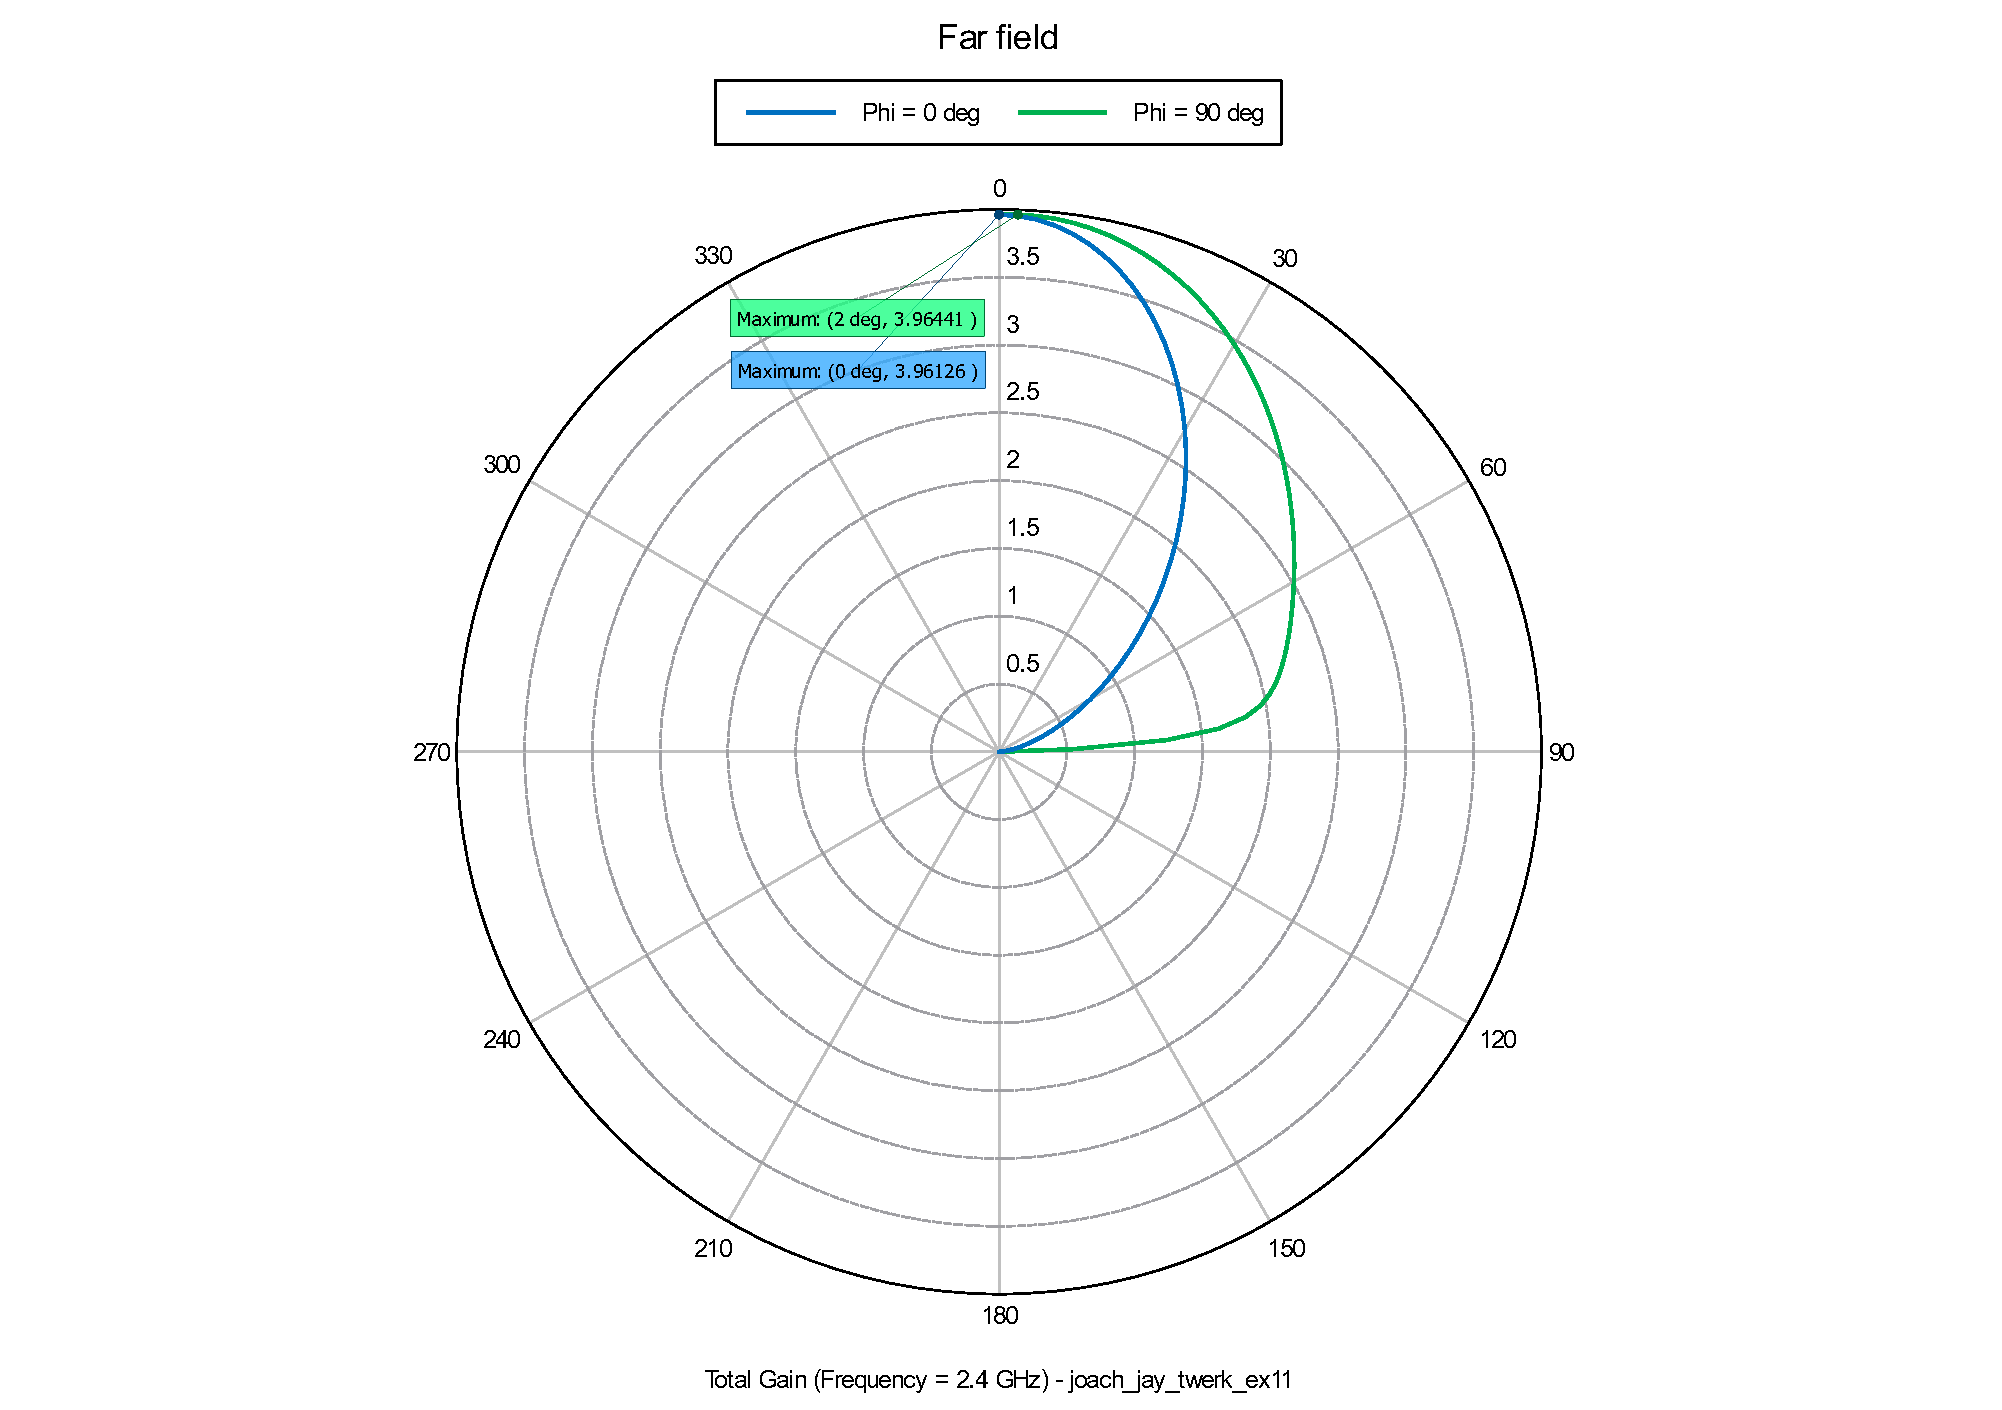
\includegraphics[width=\textwidth]{rayonnement11_annotation.pdf}
  \caption{Diagramme de rayonnement du gain [généré avec PostFeko]\label{fig:rayonnement_11}}
\end{figure}
Pour les deux valeurs de $\phi$, la directivité maximale est de \SI{0}{\degree}.

Nous nous sommes aussi intéressés au coefficient de réflexion de l'antenne ainsi qu'à sa fréquence de résonance.
\begin{figure}[htbp]
  \centering
  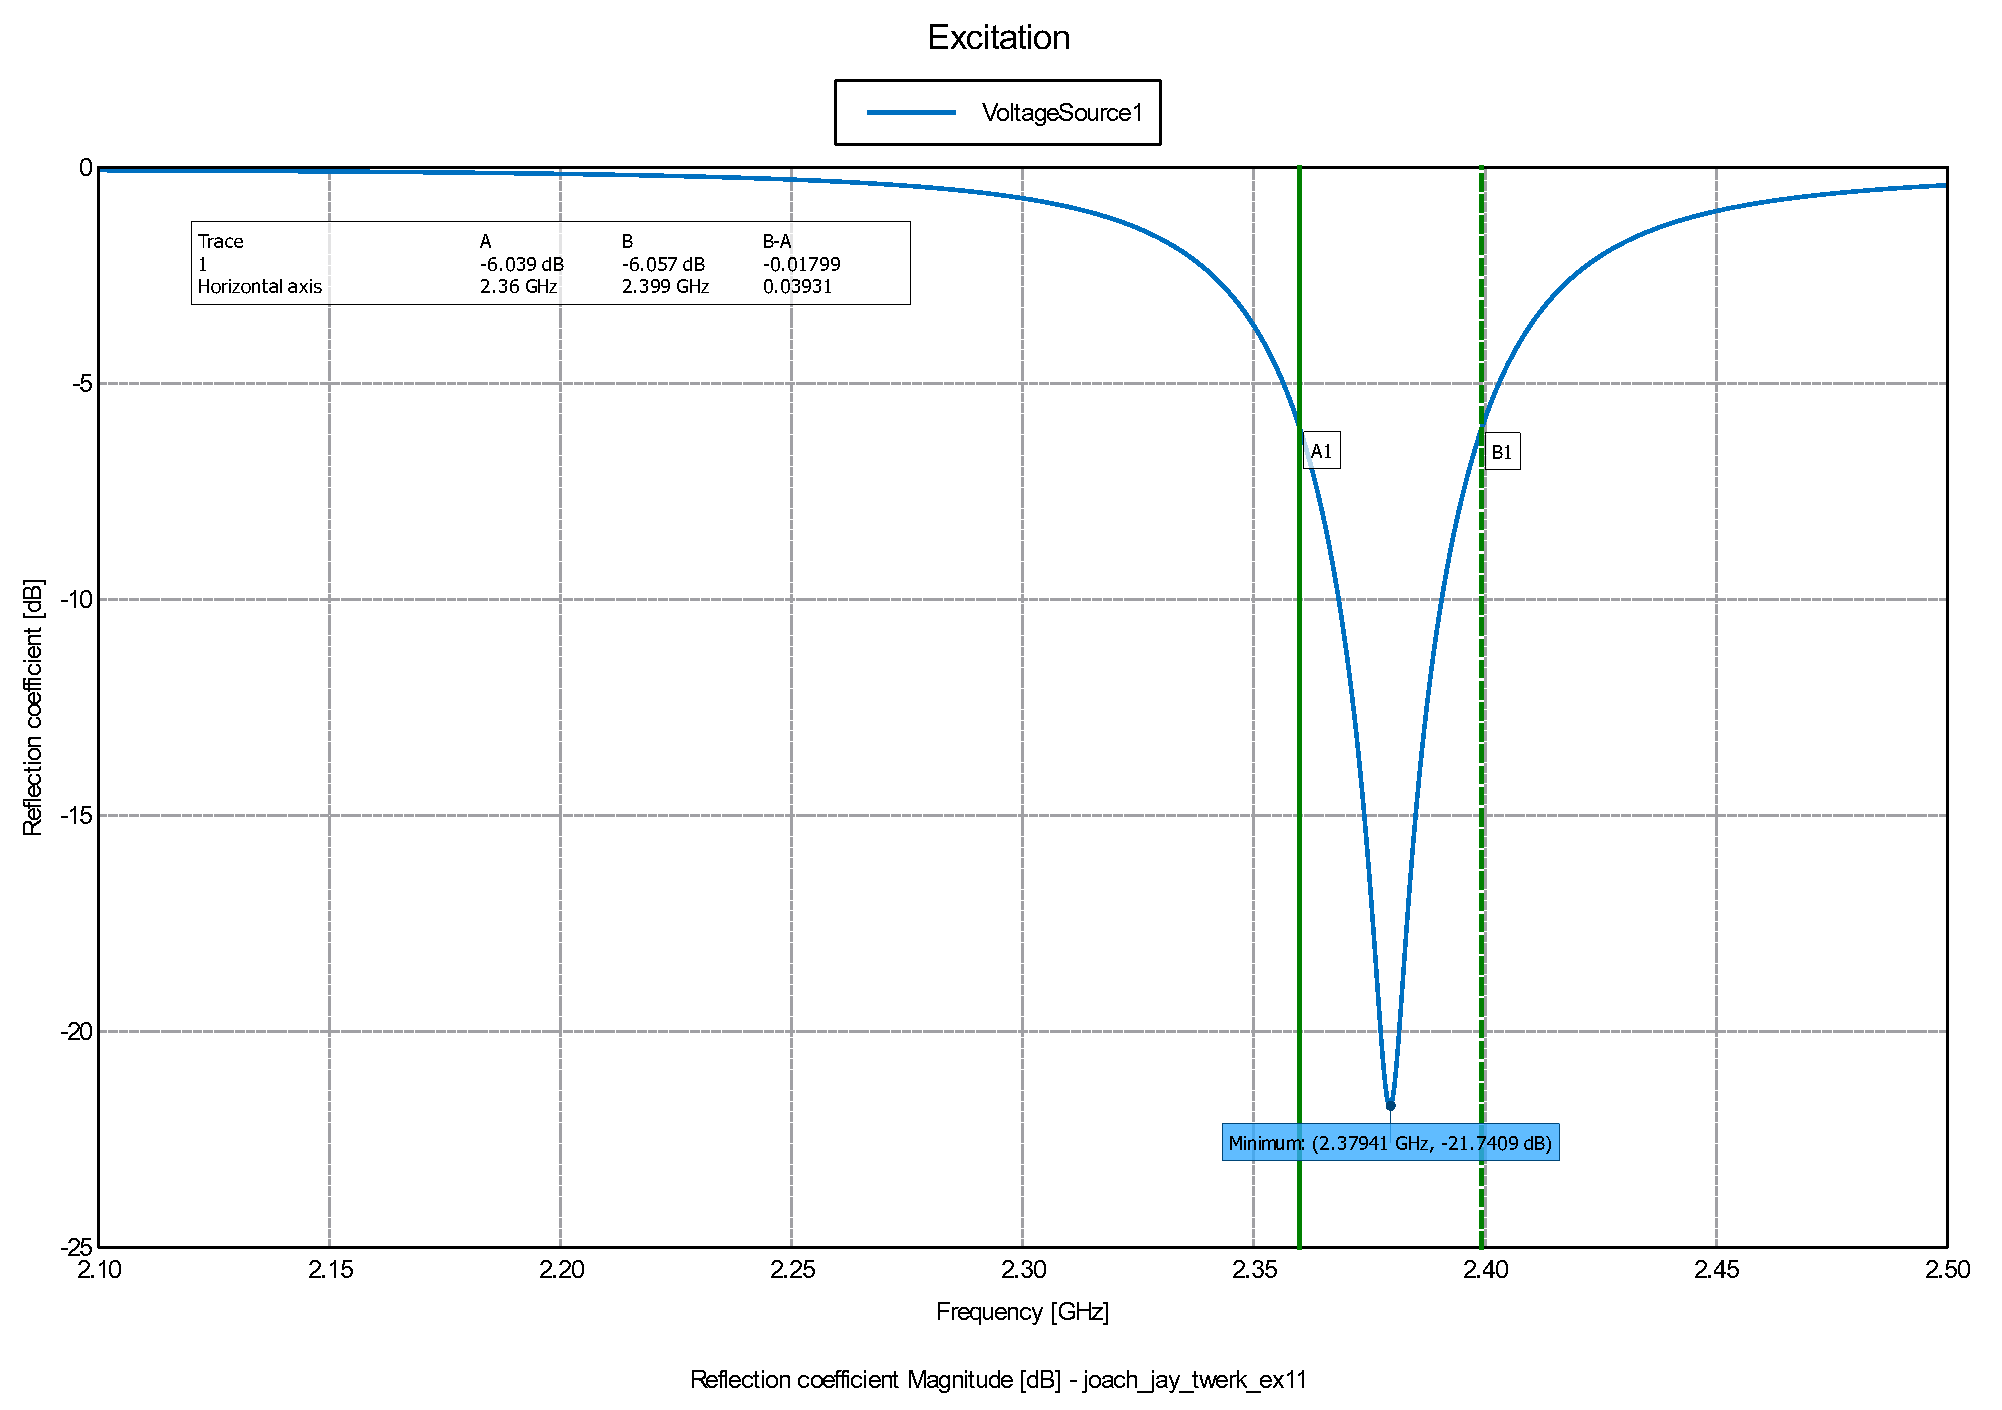
\includegraphics[width=\textwidth]{reflection11_annotation.pdf}
  \caption{Coefficient de réflexion en fonction de la fréquence [généré avec PostFeko]\label{fig:reflection11_}}
\end{figure}
La figure \ref{fig:reflection11_} nous montre que la résonance de l'antenne se situe à \SI{2.37941}{\giga\hertz} qu'à cette fréquence le coefficient de réflexion vaut \SI{-21.8}{\deci\bel}. A \SI{2.4}{\giga\hertz} ce coefficient vaut \SI{-6}{\deci\bel}, il est intéressant de noter la valeur de la bande passante définie à \SI{-6}{\deci\bel} qui vaut ici pas loin de \SI{0.04}{\giga\hertz}. Un dernier aspect important pour ce point est le pourcentage de puissance délivrée à l'antenne à la fois à la fréquence de résonance et à \SI{2.4}{\giga\hertz}. Ce pourcentage nous est donné par la formule \ref{eqn:puissance délivrée}, ce qui nous donne une valeur de \SI{99.3}{\percent} à la fréquence de résonance et \SI{75.2}{\percent} à \SI{2.4}{\giga\hertz}.
\begin{equation}
\frac{P_L}{P_{in}} = 1-\Gamma_L^2
\label{eqn:puissance délivrée}
\end{equation}

%Note pour jojol: coeff de réflection c'est gamma majuscule, aka \Gamma_L (L pour load).
%Merci d'utiliser \SI! c'est vachement cool!
%Je me suis planté, la proportion absorbée c'est 1-(gamma)². Je m'occupe (ou me suis occupé) de corriger dans ce qui est déjà fait.


\section{Simulation d'antennes filaires}
\subsection{Le dipôle court: $l \ll \lambda$}
Le gain de l'antenne dans le plan E est représenté dans la figure \ref{fig:gain21}.
\begin{figure}[htbp]
  \centering
  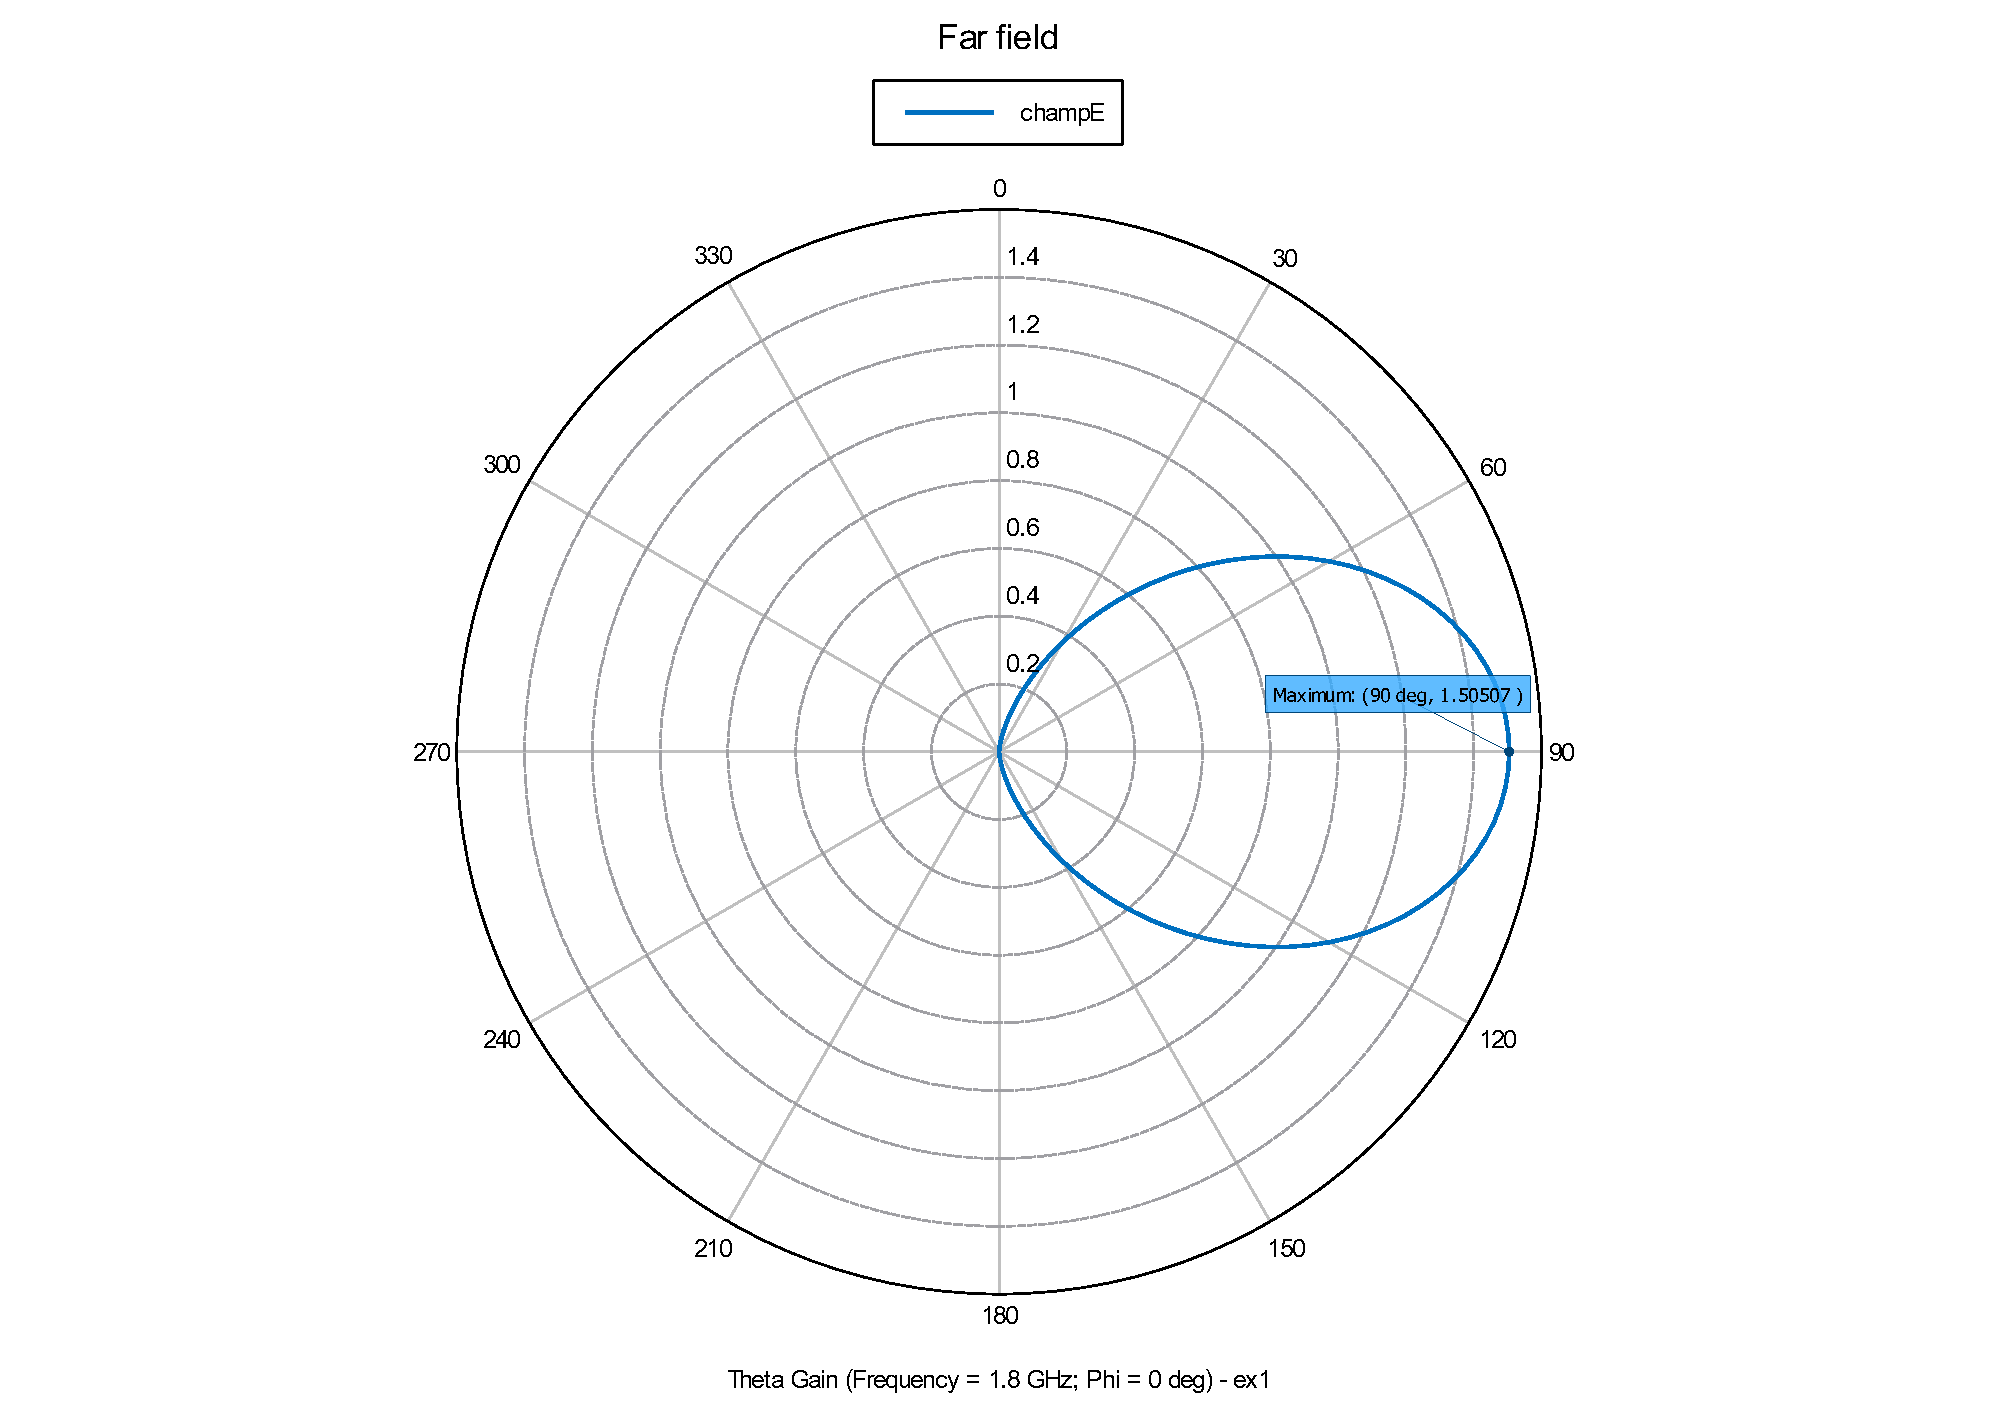
\includegraphics[width=\textwidth]{gain21.pdf}
  \caption{Diagramme de rayonnement du dipôle court dans le plan E.\label{fig:gain21}}
\end{figure}
Le gain n'est pas représenté pour $\SI{180}{\degree}<\theta<\SI{360}{\degree}$, ce qui n'est pas important puisque l'on sait que le problème présente une symétrie cylindrique. Pour la même raison, les diagrammes dans le plan H ne sont pas donnés ici, mais se déduisent logiquement de la figure \ref{fig:gain21}: le gain est indépendant de $\phi$. Sa composante $\theta$ vaut la gain maximal du diagramme de rayonnement dans le plan E, et sa composante $\phi$ vaut $0$.

Sur la figure \ref{fig:gain21}, on lit un gain maximal de $\num{1.51} = \SI{1.79}{\deci\bel}$, ce qui est légèrement supérieur à la valeur $\frac{3}{2} = \SI{1.76}{\deci\bel}$ prédite par l'approximation du dipôle de Hertz. Ceci est logique puisque la directivité maximale augmente lorsqu'on augmente la longueur du dipôle.

La résistance de rayonnement est représentée en fonction de la fréquence à la figure \ref{fig:Rar21}.
\begin{figure}[htbp]
  \centering
  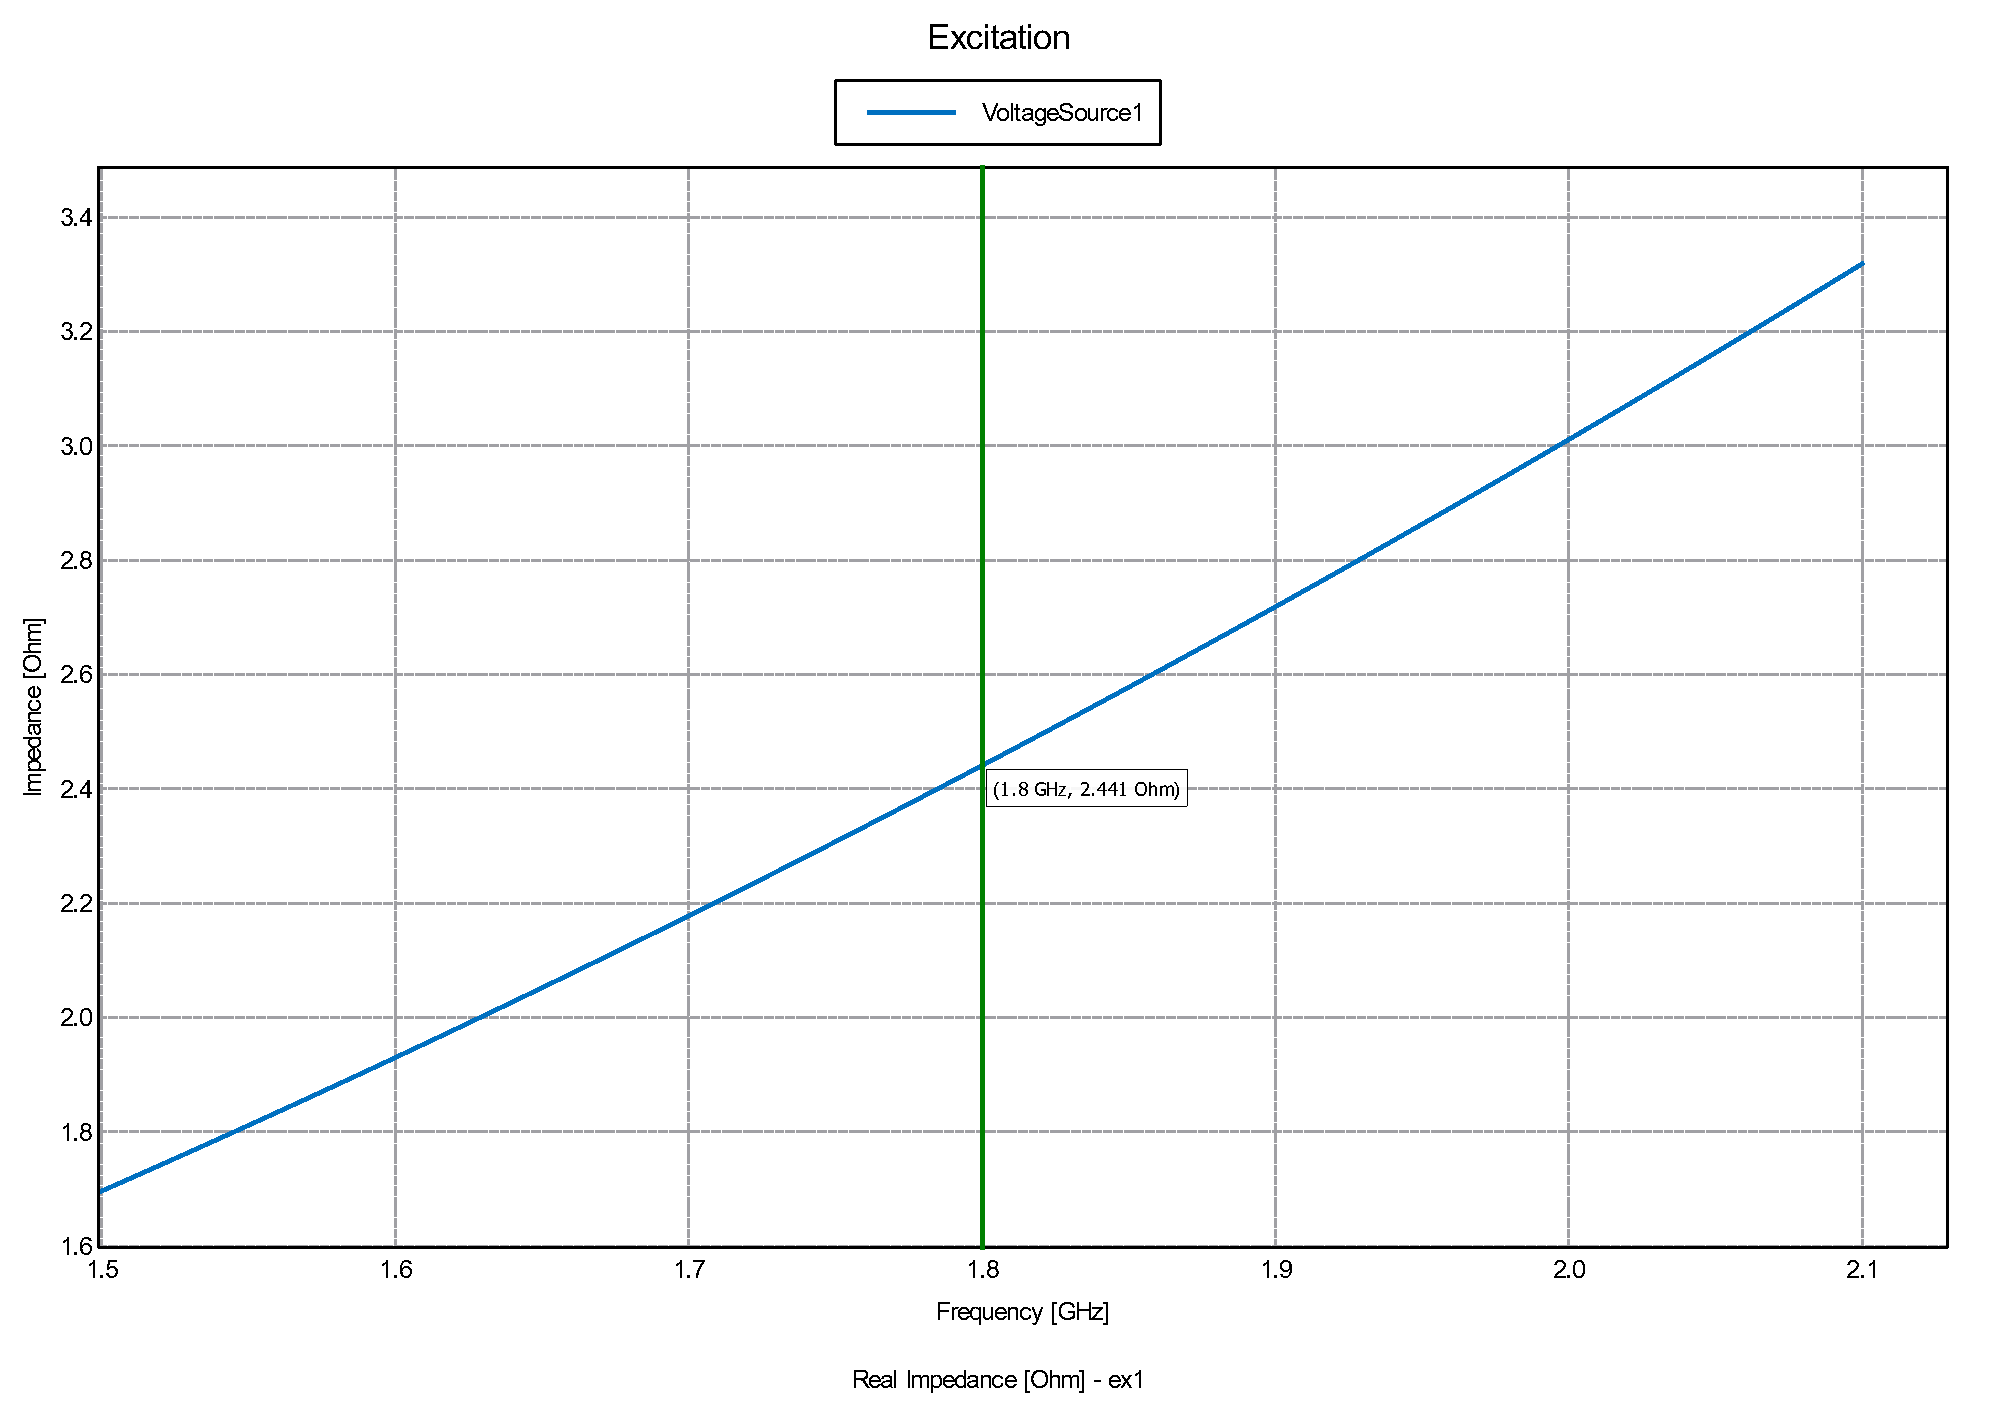
\includegraphics[width=\textwidth]{Rar21.pdf}
  \caption{Résistance de rayonnement du dipôle court en fonction de la fréquence.\label{fig:Rar21}}
\end{figure}
Puisque le fil est modélisé par un conducteur parfait et que les connections ne sont pas prises en compte, la résistance ohmique est considérée comme nulle. Sur la figure \ref{fig:Rar21}, on lit $R_{ar} = \SI{2.44}{\ohm}$ pour $f = \SI{1.8}{\giga\hertz}$, ce qui est très inférieur à la valeur $R_{ar} = 80 \left (\frac{\pi l}{\lambda} \right ) ^2 = \SI{7.90}{\ohm}$ prédite par l'approximation de l'élément de courant.

A partir de cette valeur, on obtient la fraction de puissance consommée par l'antenne en calculant d'abord $\Gamma_L$ puis en utilisant la relation \ref{eqn:puissance délivrée}.
\begin{align*}
\Gamma_L = \frac{Z_L - Z_c}{Z_L + Z_c} &= 0.91\numberthis\label{eqn:reflect}\\
\frac{P_L}{P_{in}} &= \SI{17.7}{\percent}
\end{align*}
L'adaptation d'impédance est donc très mauvaise. Ceci peut-être résolu en utilisant un dipôle demi-onde, comme nous le verrons dans la prochaine section.

\subsection{Le dipôle demi-onde: $l = \frac{\lambda}{2}$}
\label{subsec:demionde}
Le gain dans le plan E est représenté dans un diagramme polaire à la figure \ref{fig:gain22}.
\begin{figure}[htbp]
  \centering
  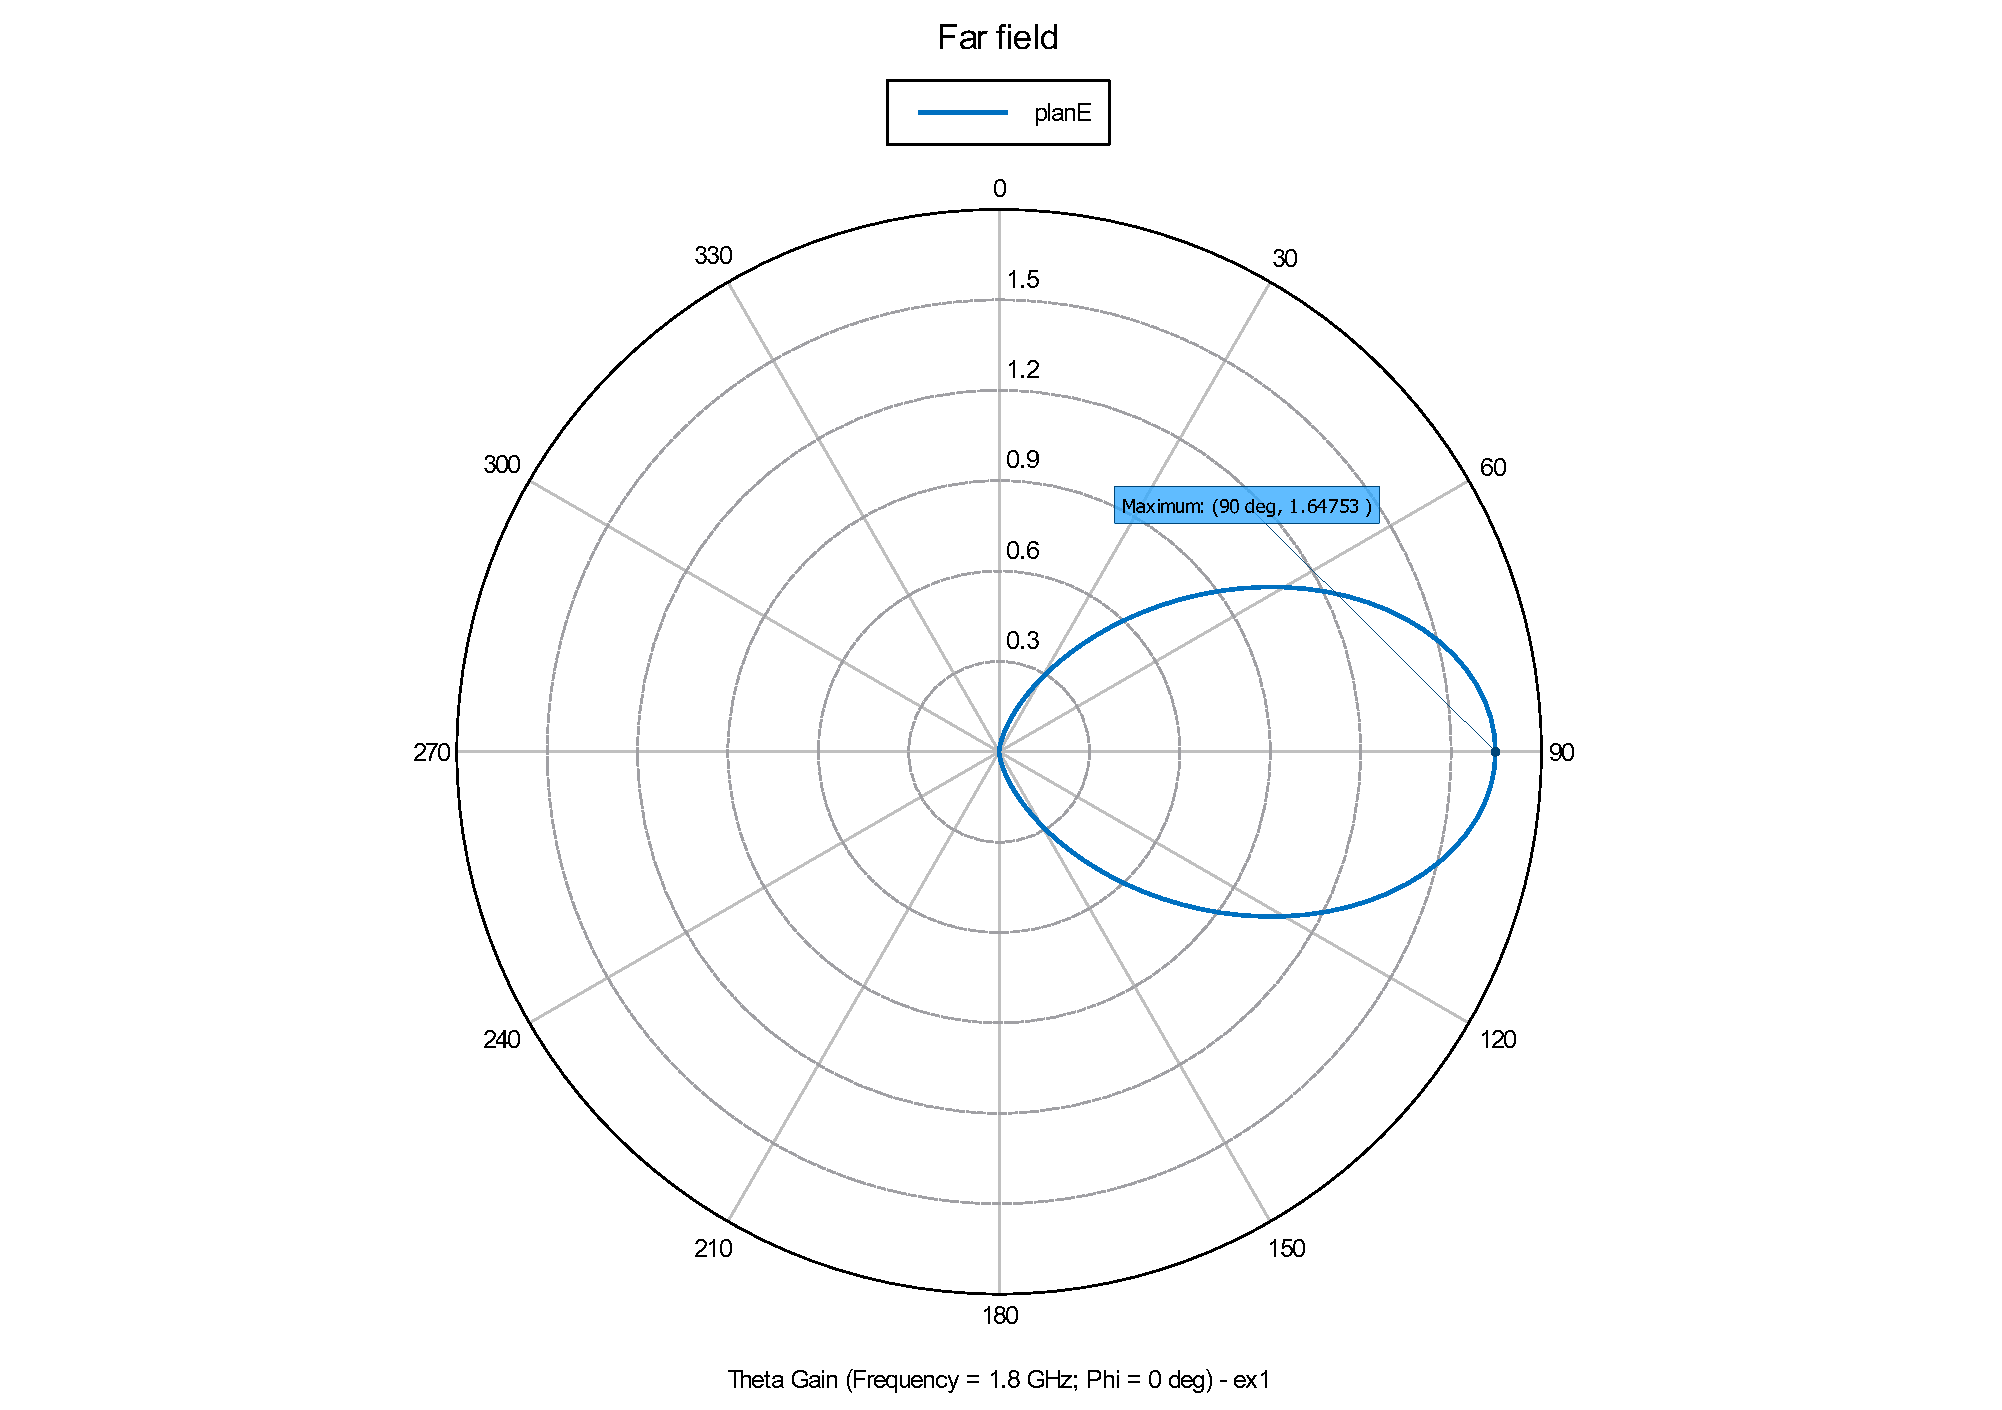
\includegraphics[width = \textwidth]{Rar22.pdf}
  \caption{Diagramme de rayonnement du dipôle demi-onde dans le plan E.\label{fig:gain22}}
\end{figure}
Les propriétés de symétrie de la figure \ref{fig:gain21} s'appliquent toujours. On lit sur le diagramme de rayonnement un gain maximal de \num{1.65}, ce qui est légèrement inférieur à la valeur de \num{1.7} prédite avec l'approximation $\left ( \frac{\cos(\frac{\pi}{2}\cos\theta)}{\sin\theta} \right ) ^2 \simeq \sin^3 \theta$.

Sur la figure \ref{fig:Z22},
\begin{figure}[htbp]
  \centering
  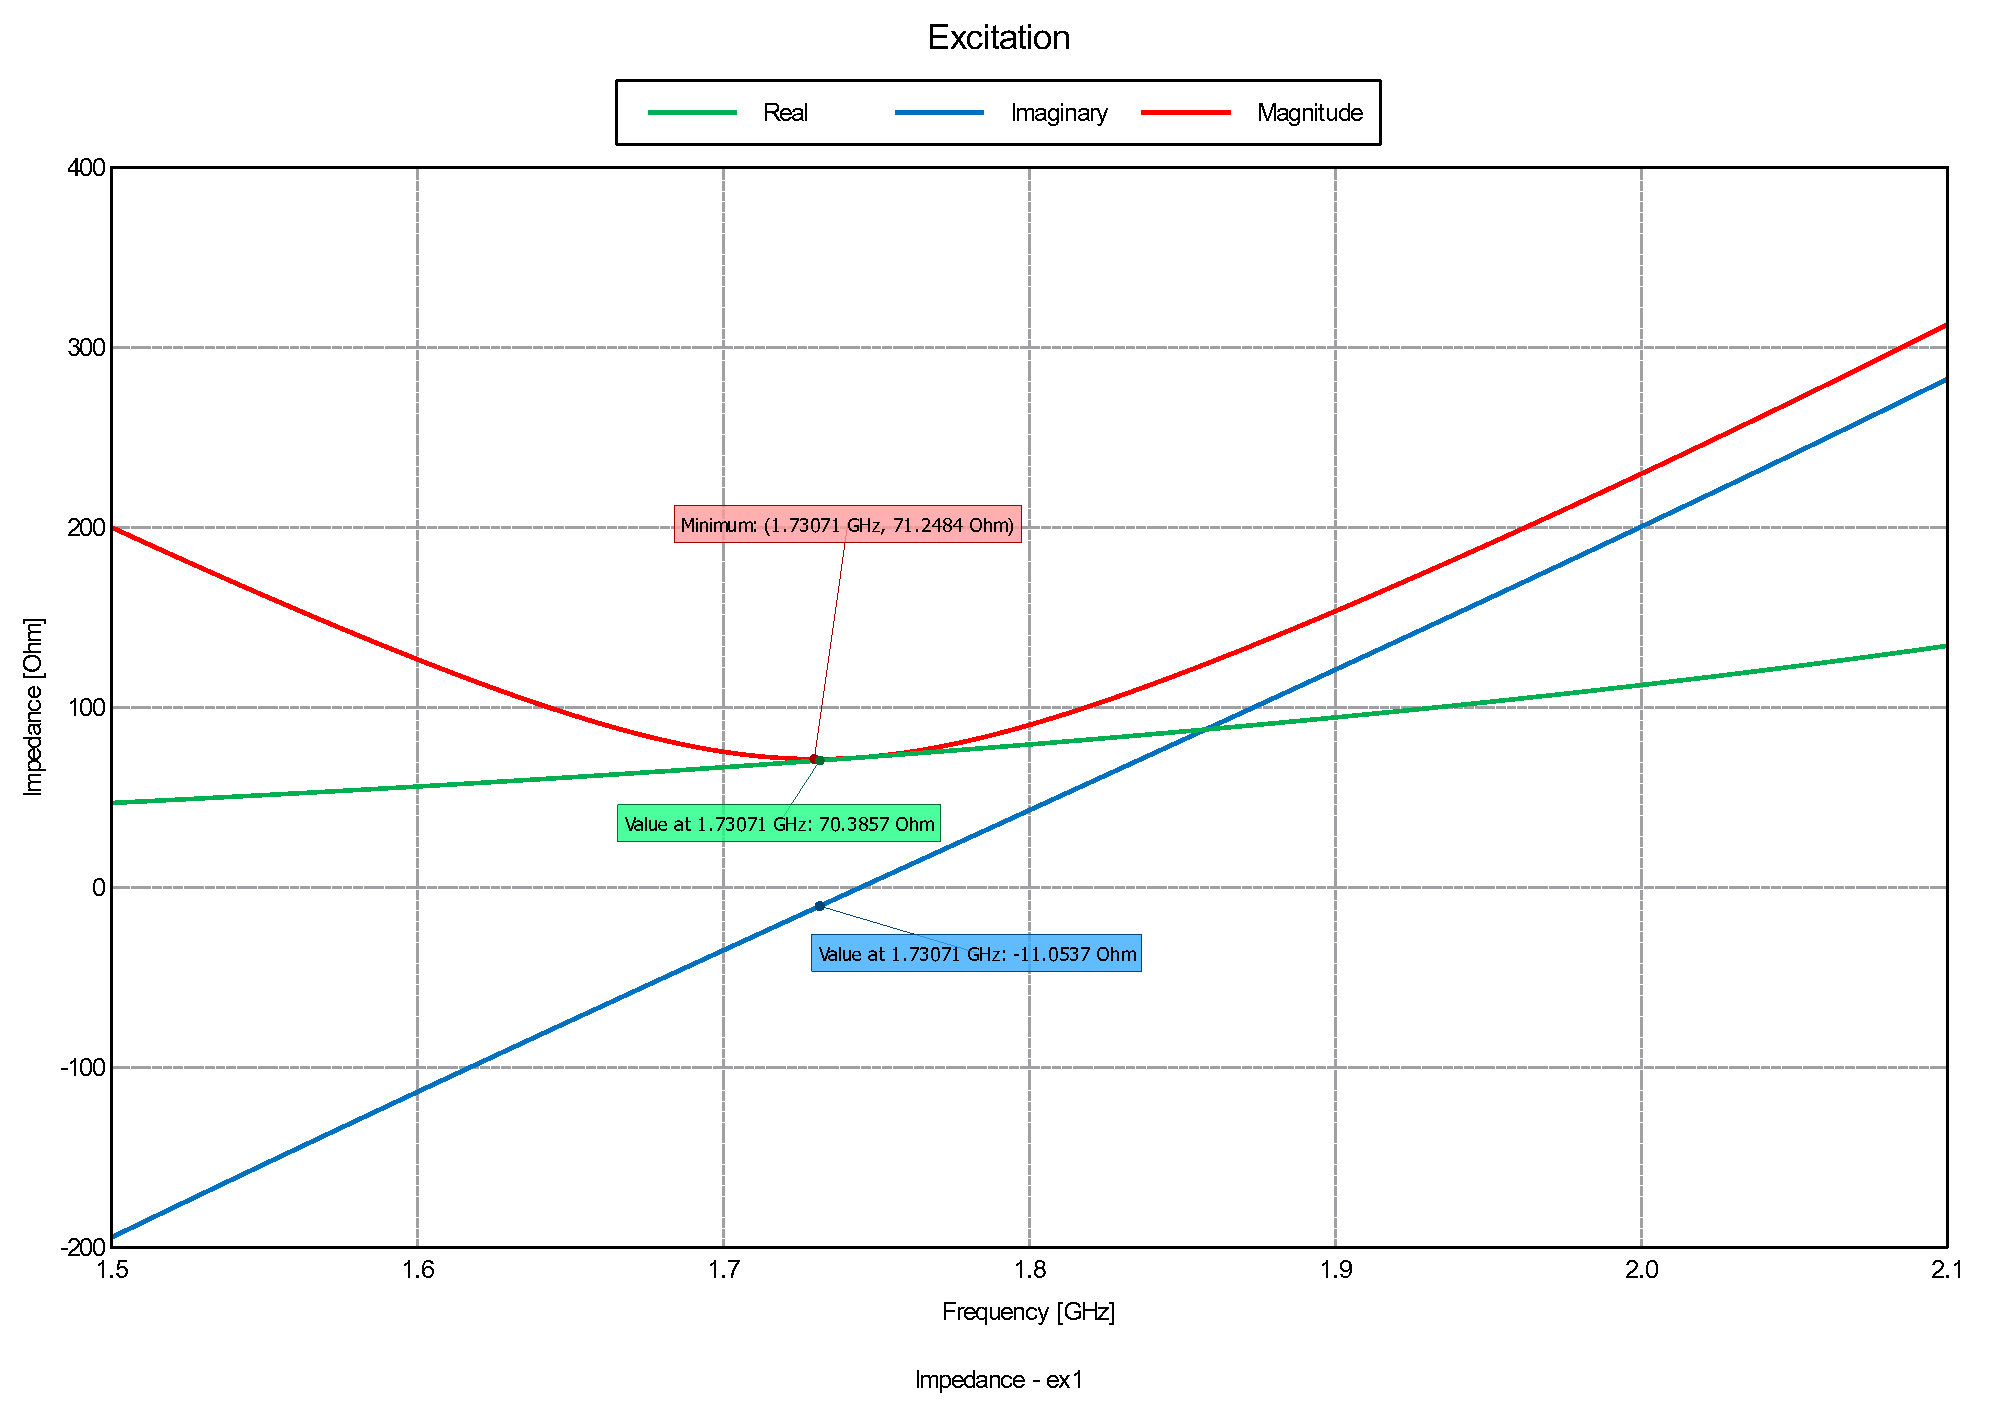
\includegraphics[width = \textwidth]{Z22.pdf}
  \caption{Parties réelle et imaginaire et module de l'impédance de l'antenne en fonction de la fréquence.\label{fig:Z22}}
\end{figure}
on constate que la partie imaginaire de l'impédance croît linéairement avec la fréquence, et ce beaucoup plus rapidement que la partie réelle qui peut est considérée comme quasi constante. De plus, comme la partie imaginaire évolue d'une valeur négative vers une valeur positive, le module de l'impédance n'est lui pas monotone et présente un minimum qui est approximativement donné par le zéro de la partie imaginaire. Sur la figure \ref{fig:Z22}, ce point se situe à \SI{1.73}{\giga\hertz}. Nous allons maintenant essayer de le déplacer à \SI{1.8}{\giga\hertz} en modifiant la longueur du dipôle.

Ceci est fait à la figure \ref{fig:Z022}.
\begin{figure}[htbp]
  \centering
  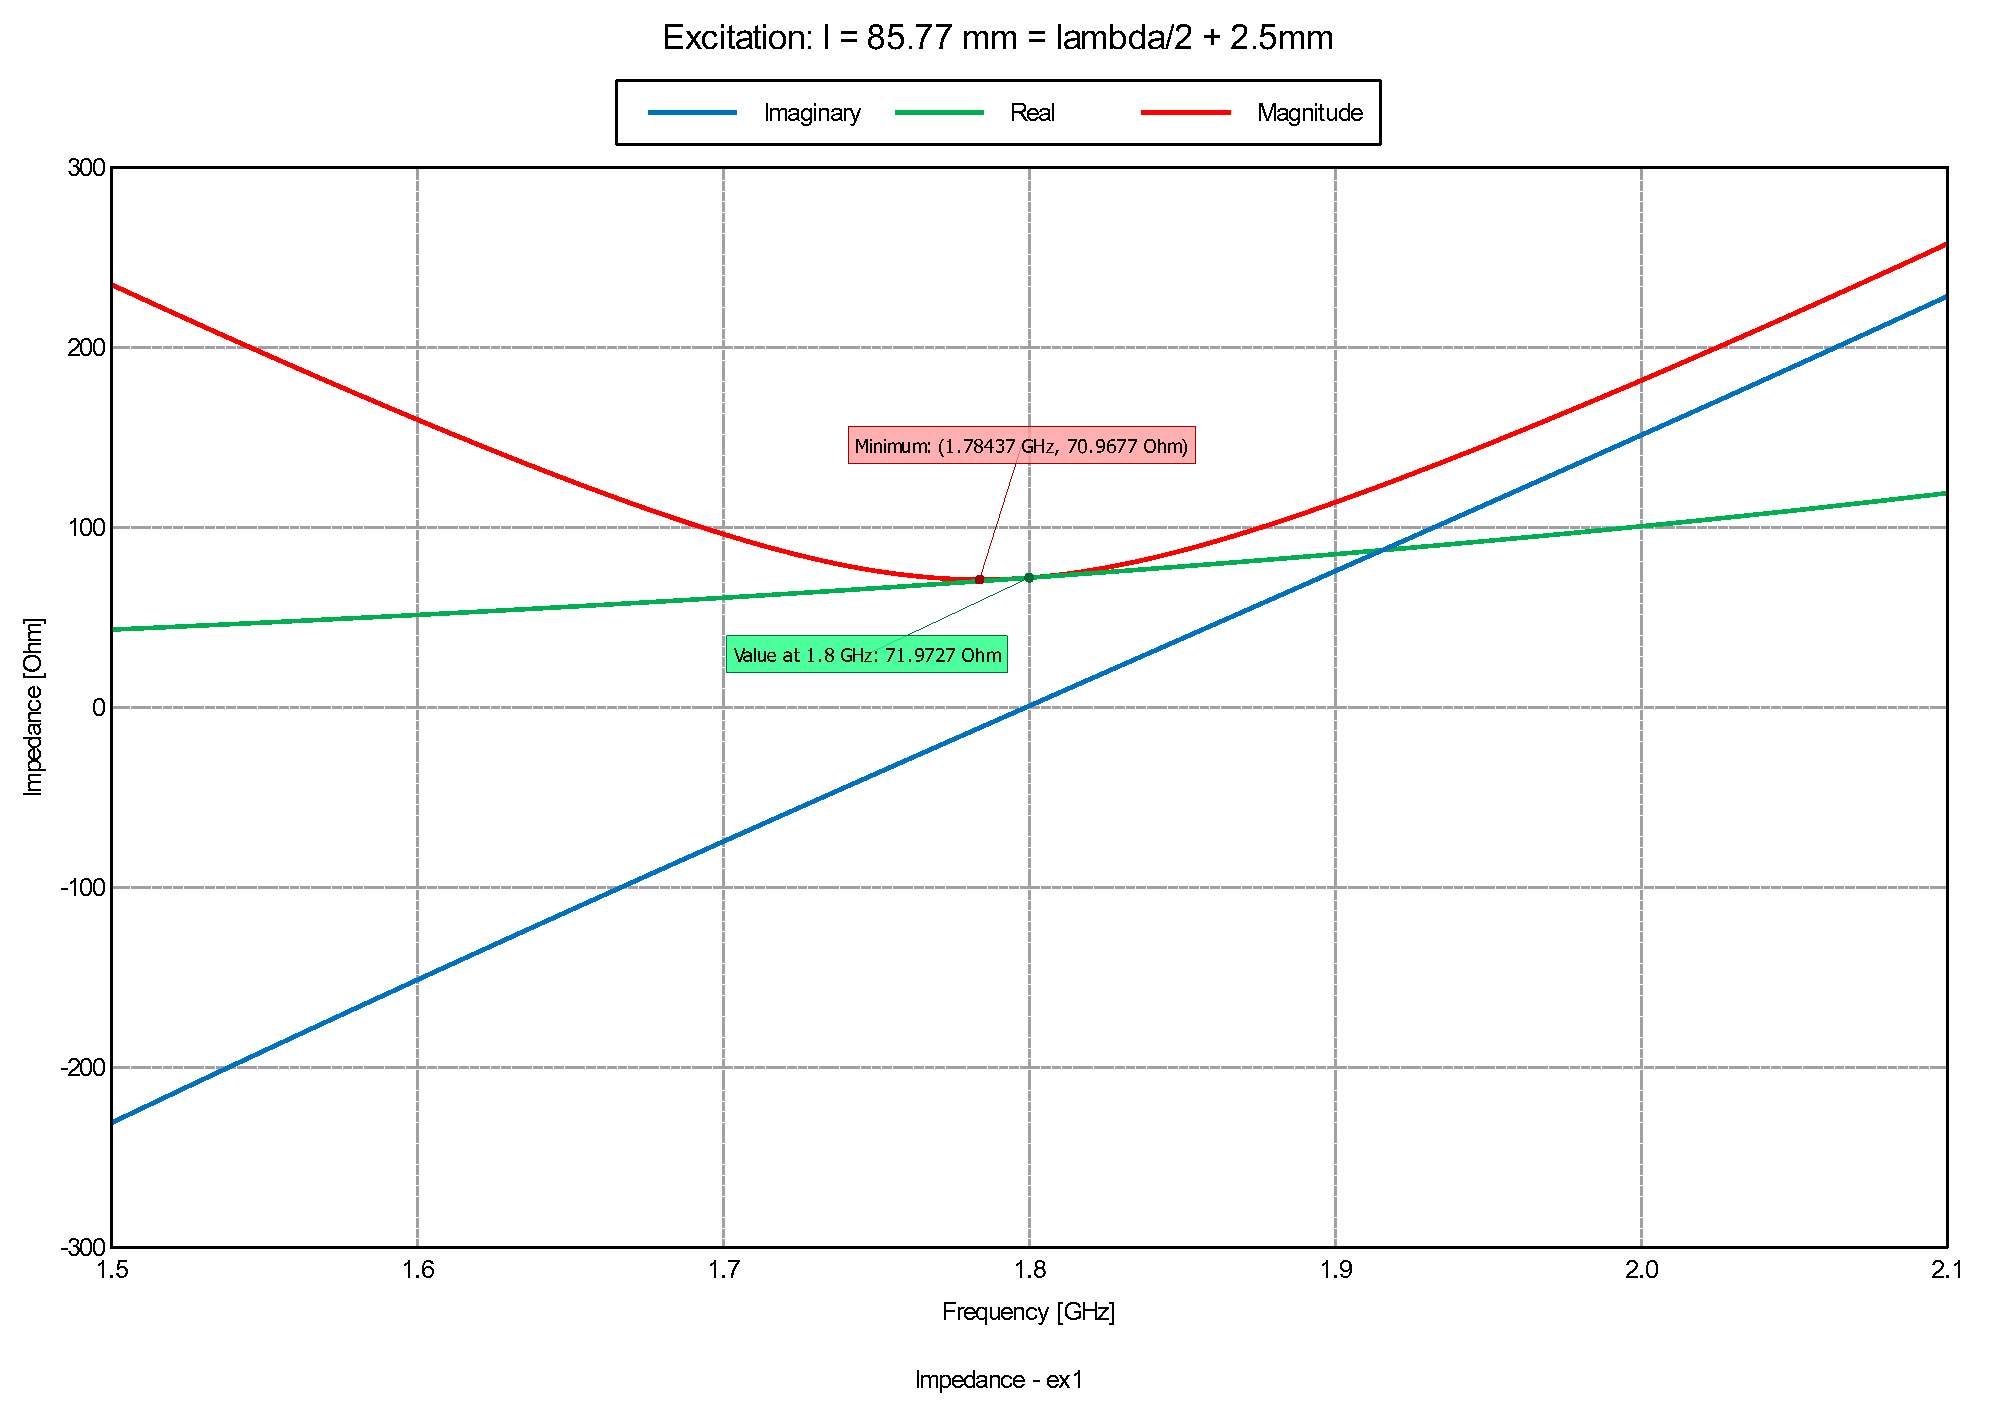
\includegraphics[width = \textwidth]{Z022.pdf}
  \caption{Parties réelle et imaginaire et module de l'impédance de l'antenne adaptée pour \SI{1.8}{\giga\hertz} en fonction de la fréquence.\label{fig:Z022}}
\end{figure}
La partie imaginaire de l'impédance s'annule bien en $f = \SI{1.8}{\giga\hertz}$ et le module de l'impédance de rayonnement est donc proche de son minimum.

En utilisant la relation \ref{eqn:reflect}, on obtient $\Gamma_L = 0.027 = \SI{-31.2}{\deci\bel}$ pour $Z_c = \SI{75}{\ohm}$. Ceci est confirmé par la simulation, comme le montre la figure \ref{fig:gamma22}.
\begin{figure}[htbp]
  \centering
  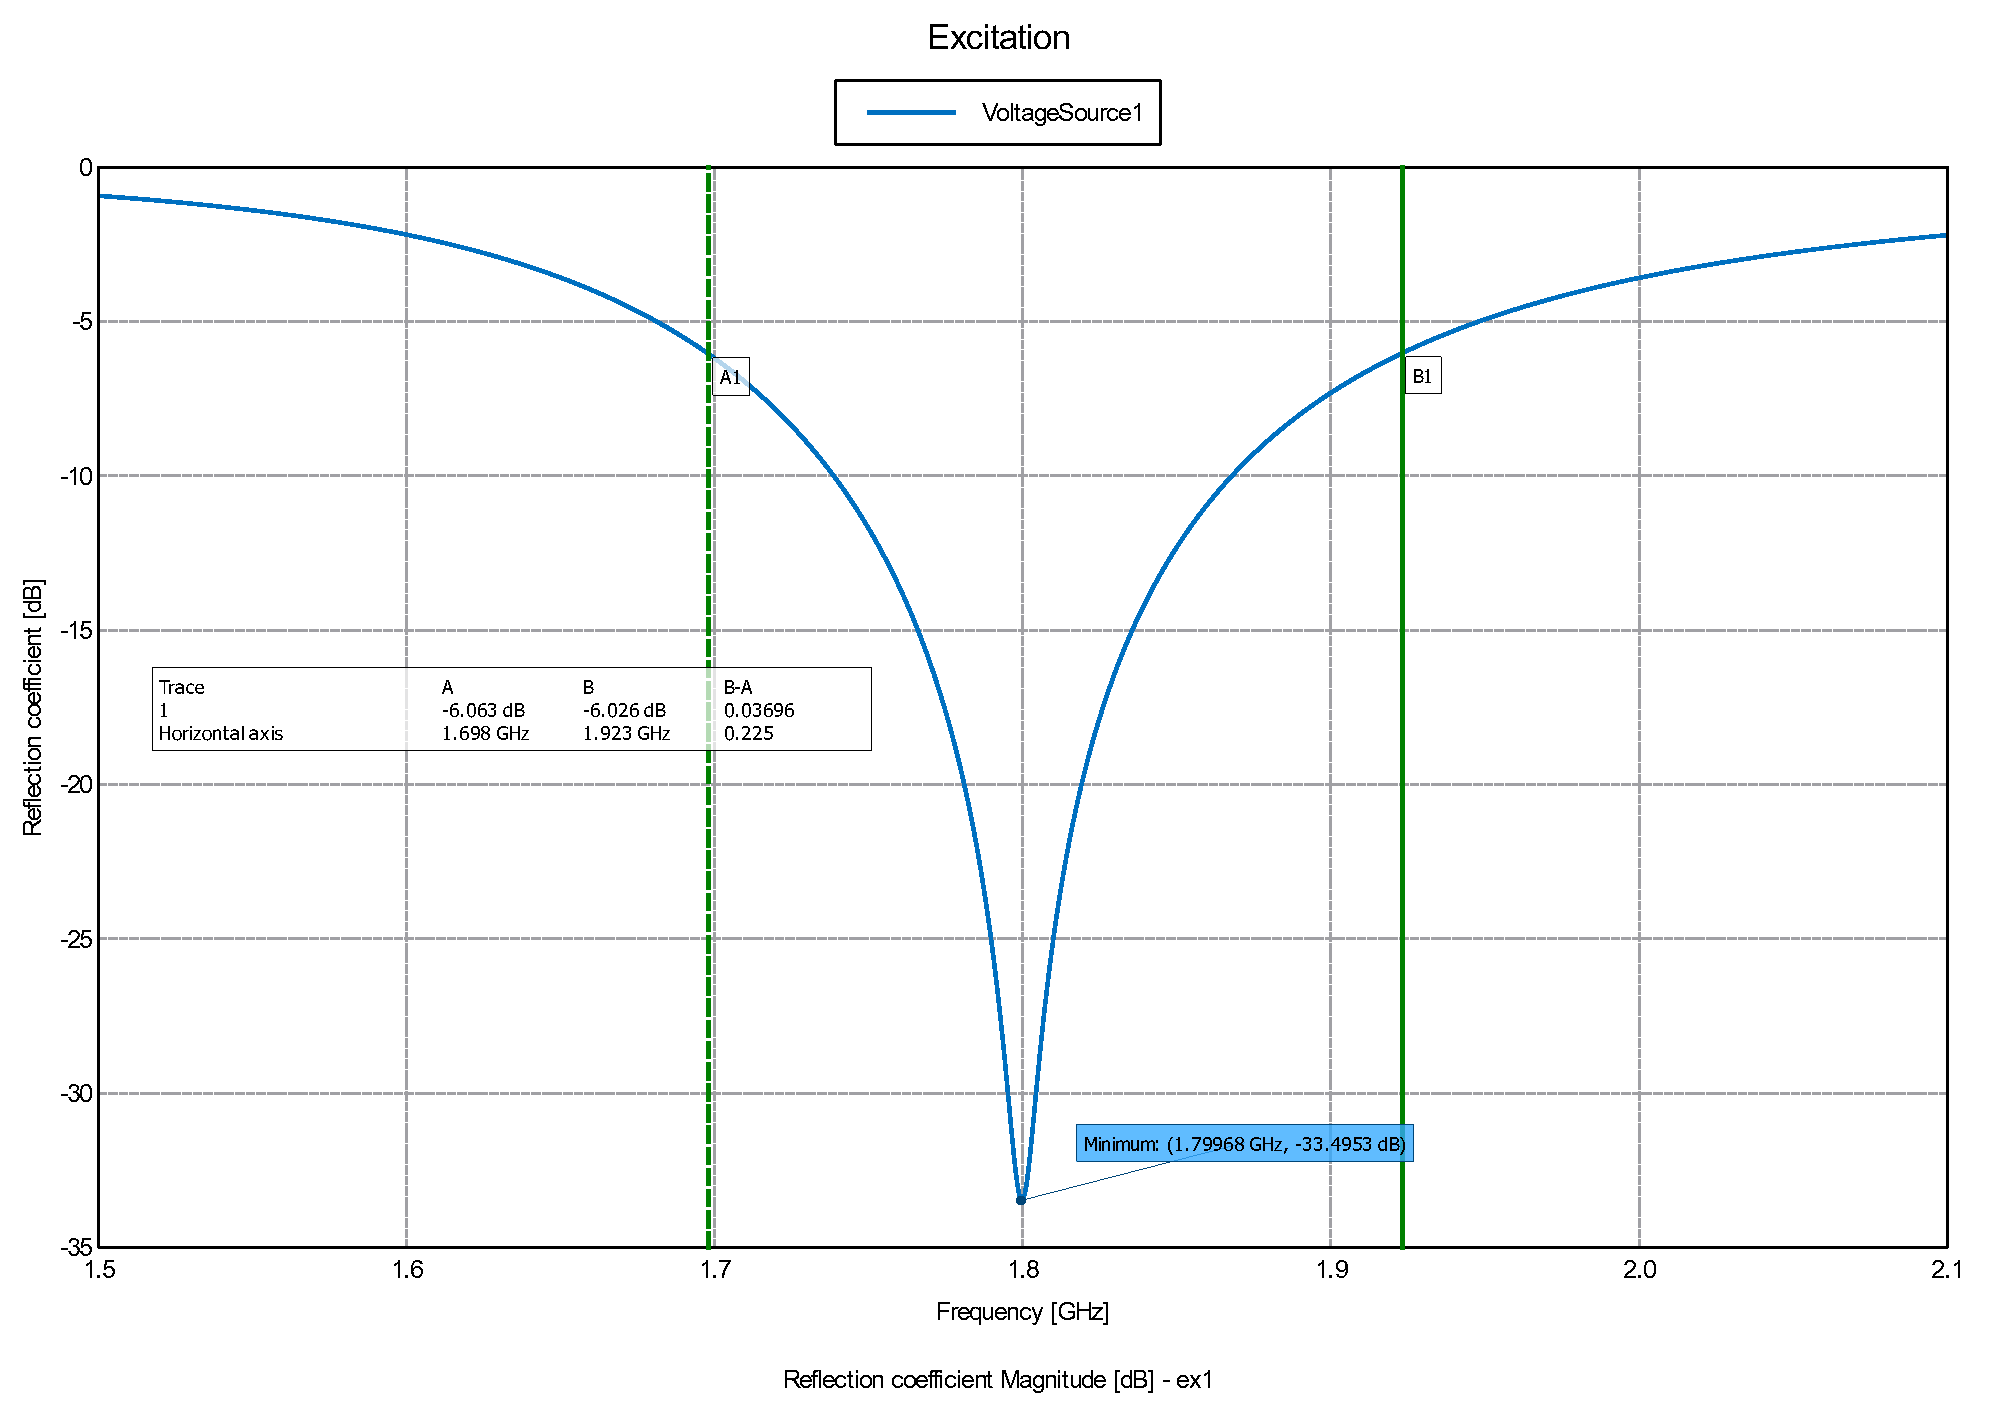
\includegraphics[width = \textwidth]{gamma22.pdf}
  \caption{$\Gamma_L$ de l'antenne dipôle adaptée pour \SI{1.8}{\giga\hertz} en fonction de la fréquence.\label{fig:gamma22}}
\end{figure}
De ce coefficient de réflexion on tire la fraction de puissance consommée à l'antenne par la relation \ref{eqn:puissance délivrée}.
\[
  \frac{P_L}{P_{in}} = \SI{99.9}{\percent}
\]

Jusqu'à présent, nous avons travaillé avec un diamètre de fil = $0.00001 \lambda$. Lorsqu'on multiplie ce diamètre par 50, on constate que la fréquence de résonance est légèrement diminuée, mais surtout que la bande passante est plus que doublée, comme le montre la figure \ref{fig:gamma5022}.
\begin{figure}[htbp]
  \centering
  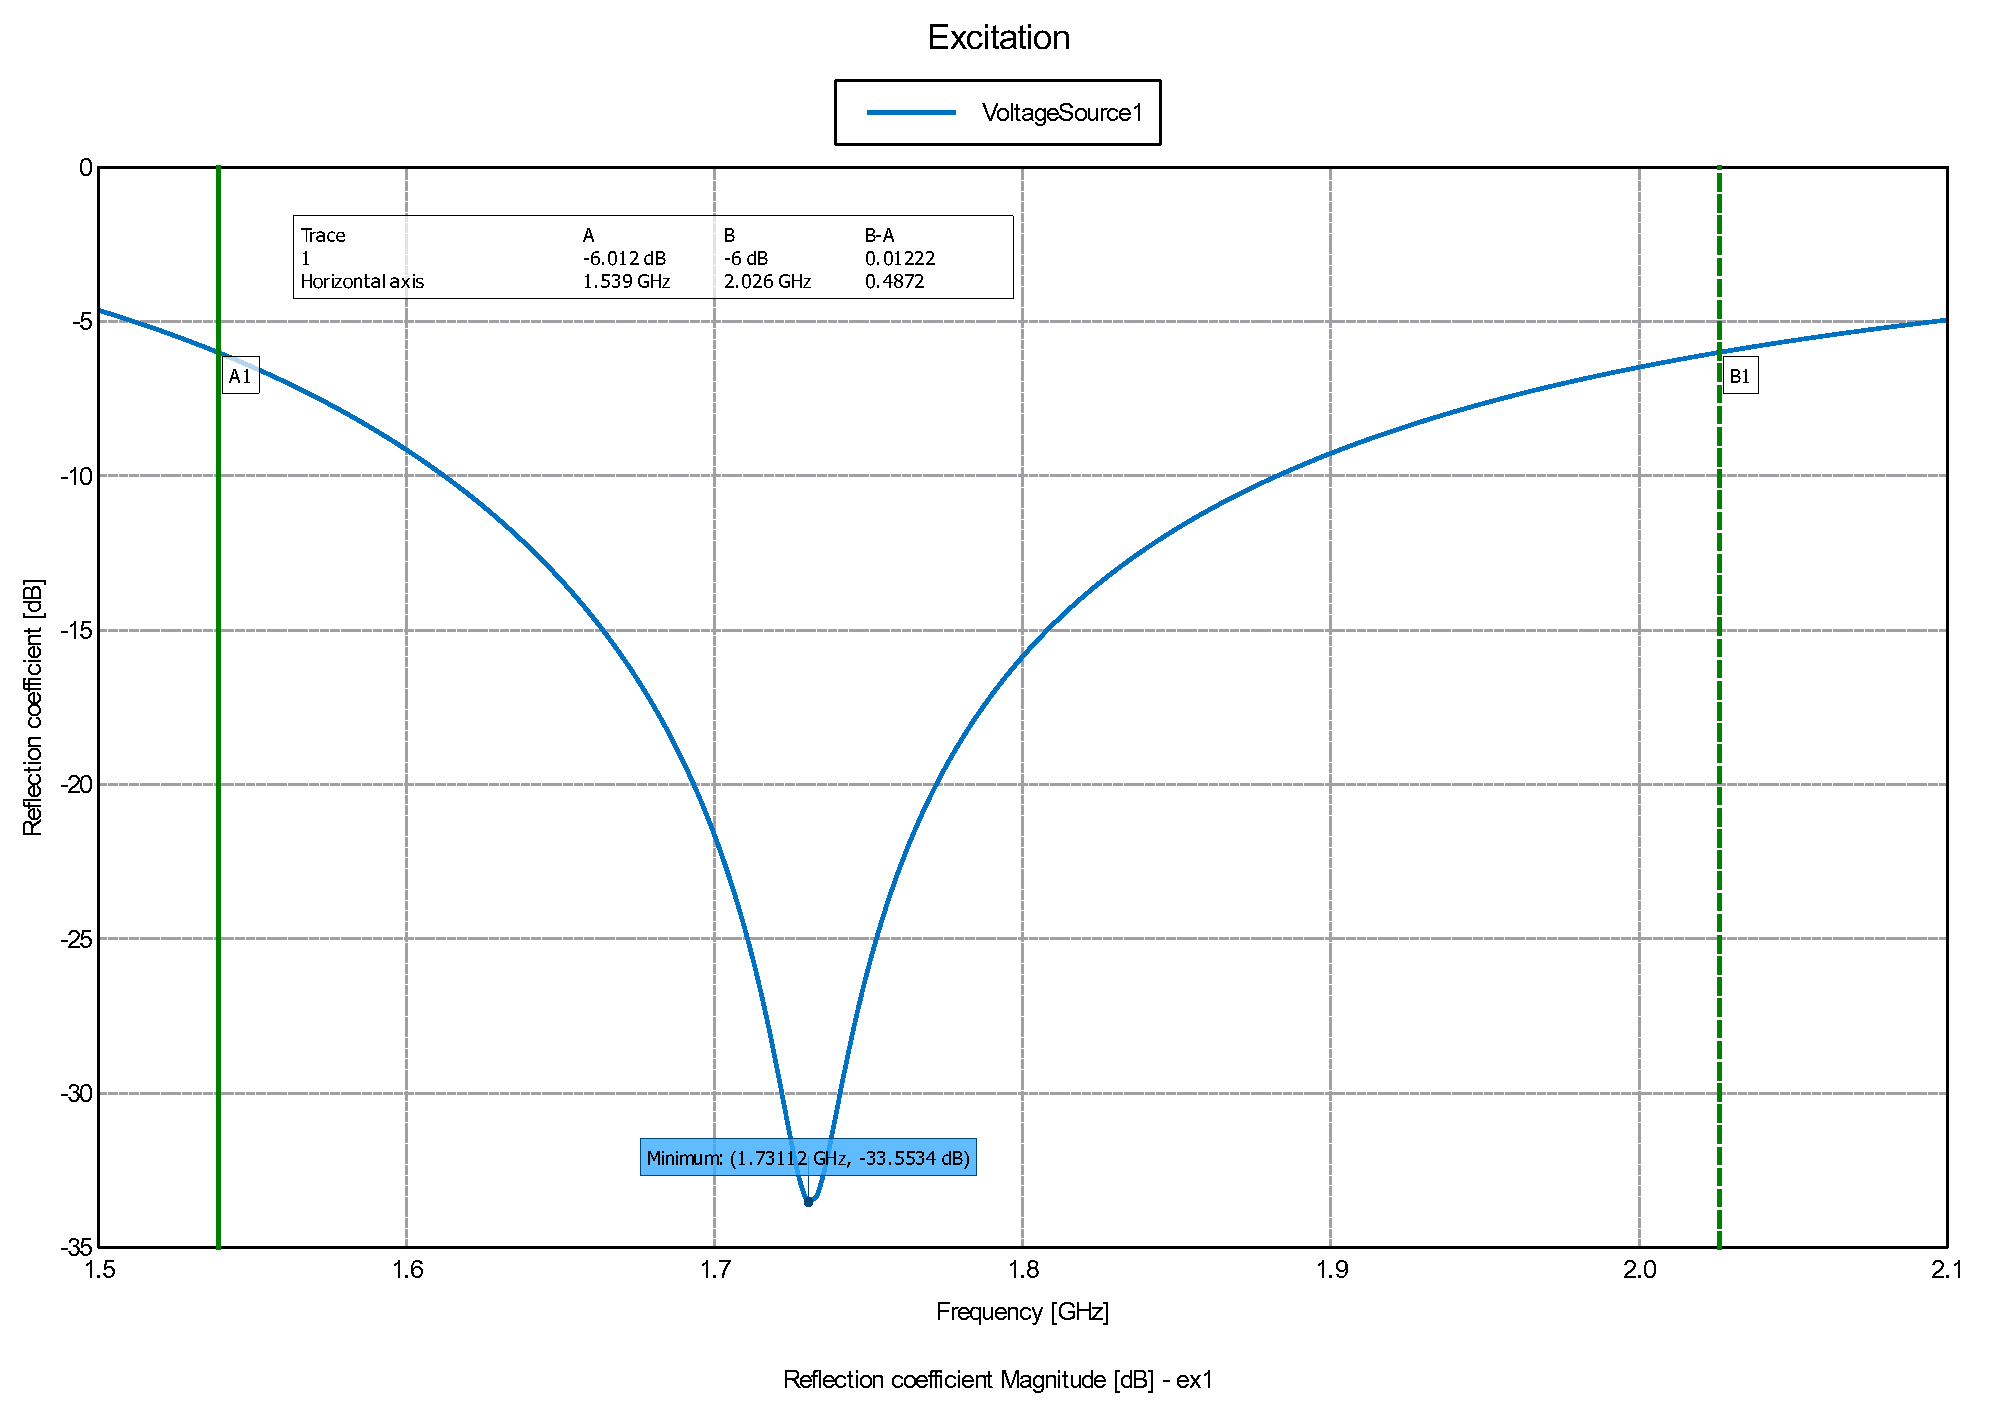
\includegraphics[width = \textwidth]{gamma5022.pdf}
  \caption{$\Gamma_L$  en fonction de la fréquence de l'antenne dipôle adaptée pour \SI{1.8}{\giga\hertz}, et diamètre multiplié par 50.\label{fig:gamma5022}}
\end{figure}
On constate en effet que la largeur de bande passe de \SI{225}{\mega\hertz} (figure \ref{fig:gamma22}) à \SI{487}{\mega\hertz} (figure \ref{fig:gamma5022}). Ceci s'explique par le fait qu'augmenter le diamètre du fil réduit la pente de $\Im(Z_L)$ en fonction de la fréquence.

\subsection{Le dipôle replié}
Le coefficient de réflexion du dipôle demi-onde replié est représenté en fonction de la fréquence à la figure \ref{fig:Z231}
\begin{figure}[htbp]
  \centering
  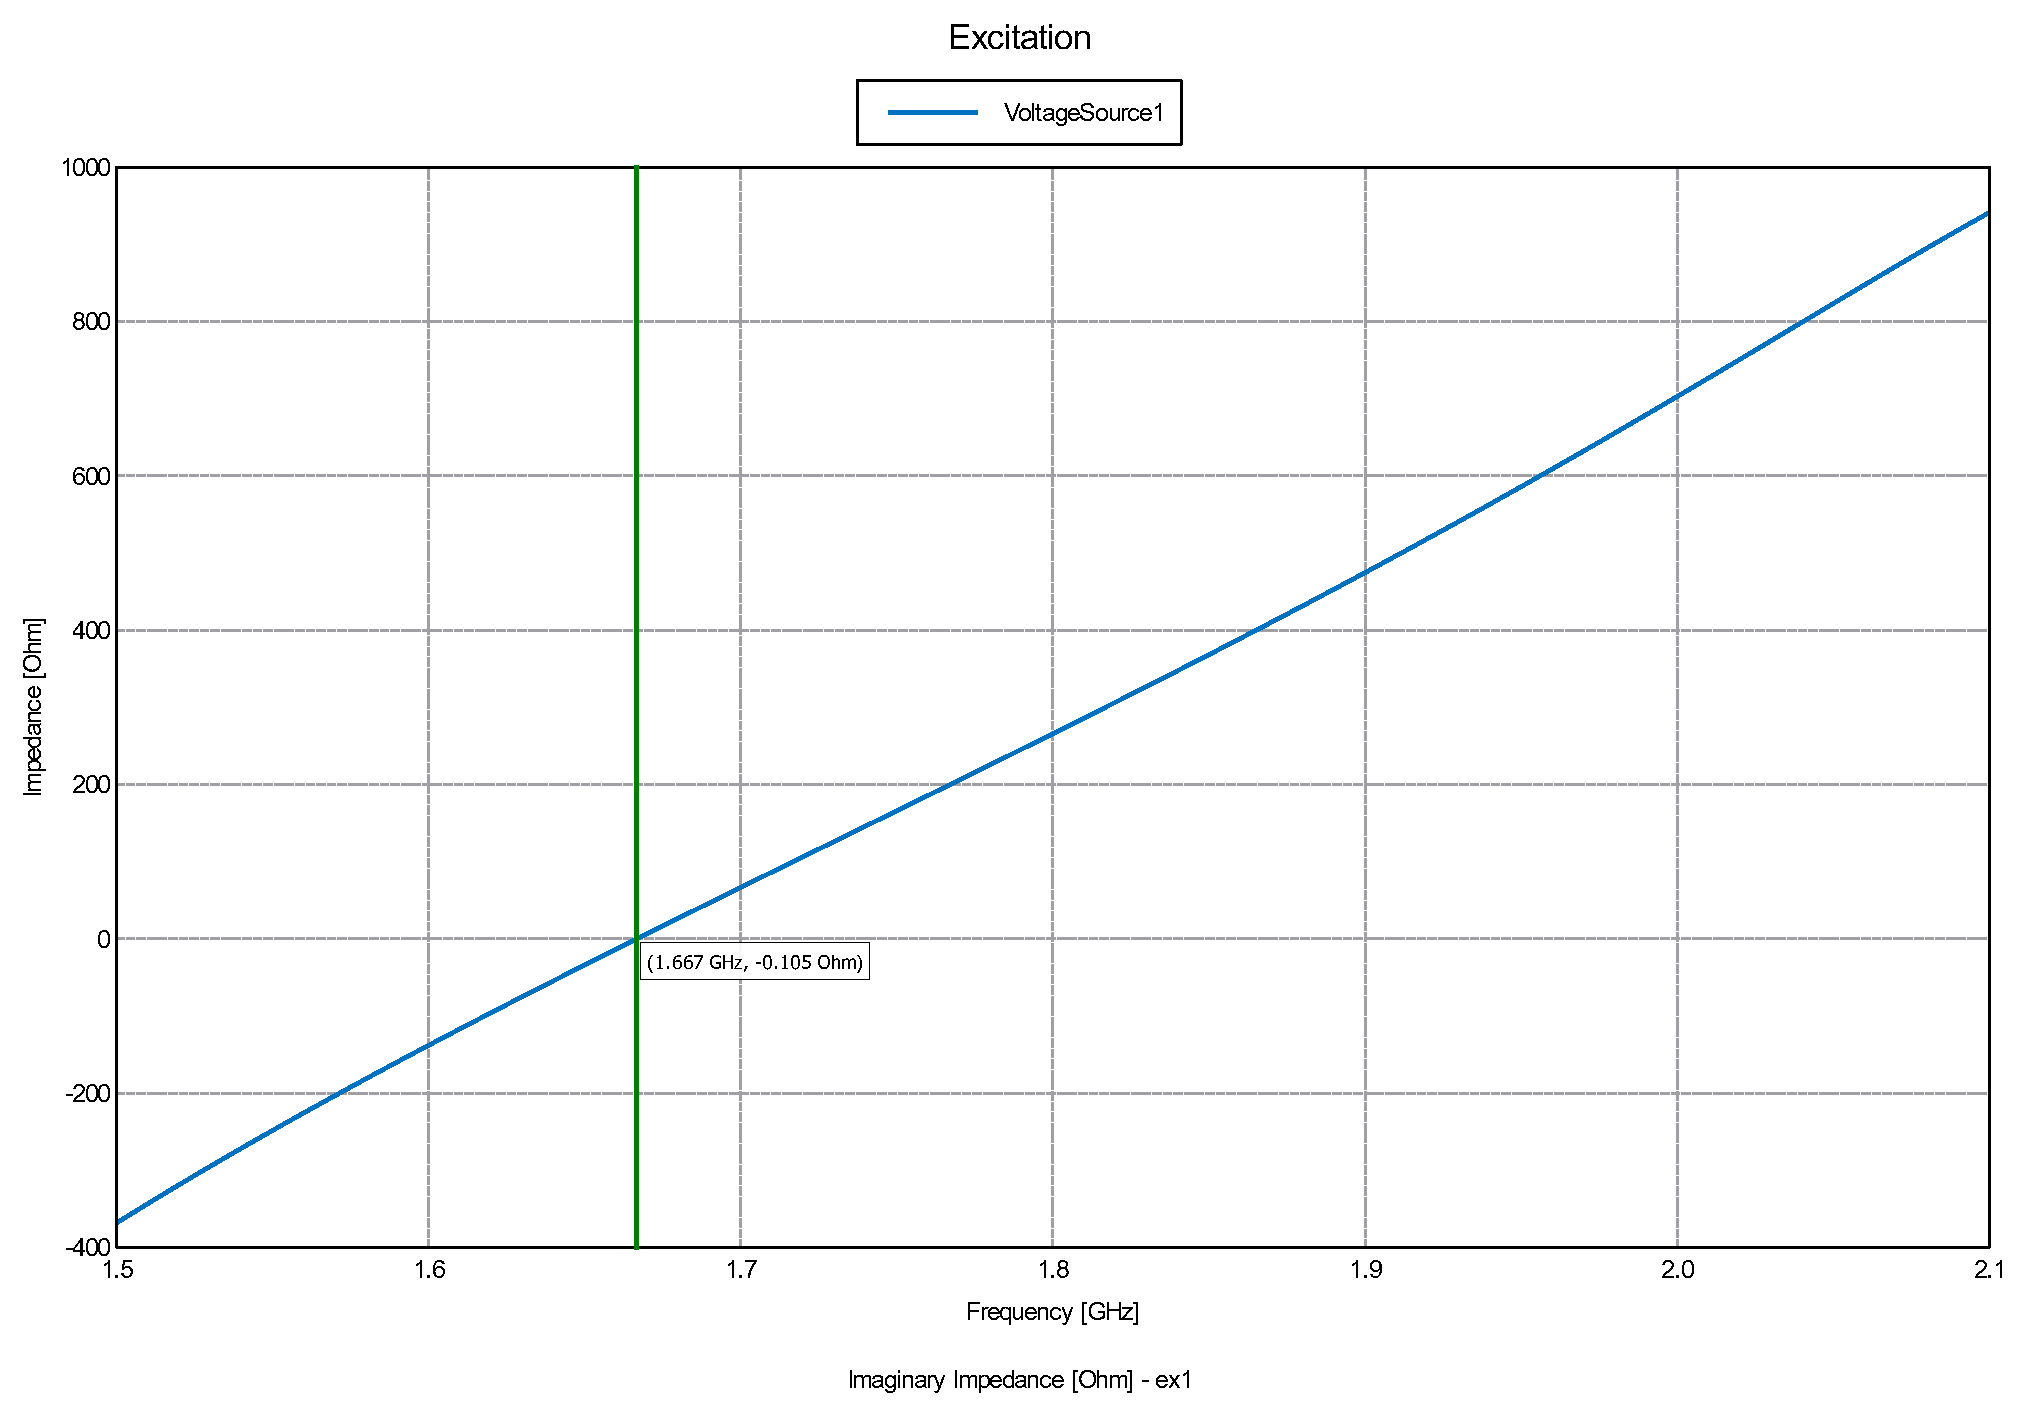
\includegraphics[width = \textwidth]{Z231.pdf}
  \caption{$\Im(Z_L)$ du dipôle demi-onde replié en fonction de la fréquence.\label{fig:Z231}}
\end{figure}
On constate que $\Im(Z_L)$ s'annule maintenant à $f = \SI{1.67}{\giga\hertz}$. Puisque $\Im(Z_L)$ évolue linéairement avec la fréquence, il suffit de remplacer le paramètre $\lambda$ dans le dimensionnement de l'antenne par $\frac{1.67}{1.8}\lambda$ pour construire un dipôle replié qui résonne effectivement autour de \SI{1.8}{\giga\hertz}. Ceci est fait à la figure \ref{fig:Z232}, qui représente la partie imaginaire de l'impédance du dipôle replié de longueur $l = 0.464 \lambda$ en fonction de la fréquence.
\begin{figure}[htbp]
  \centering
  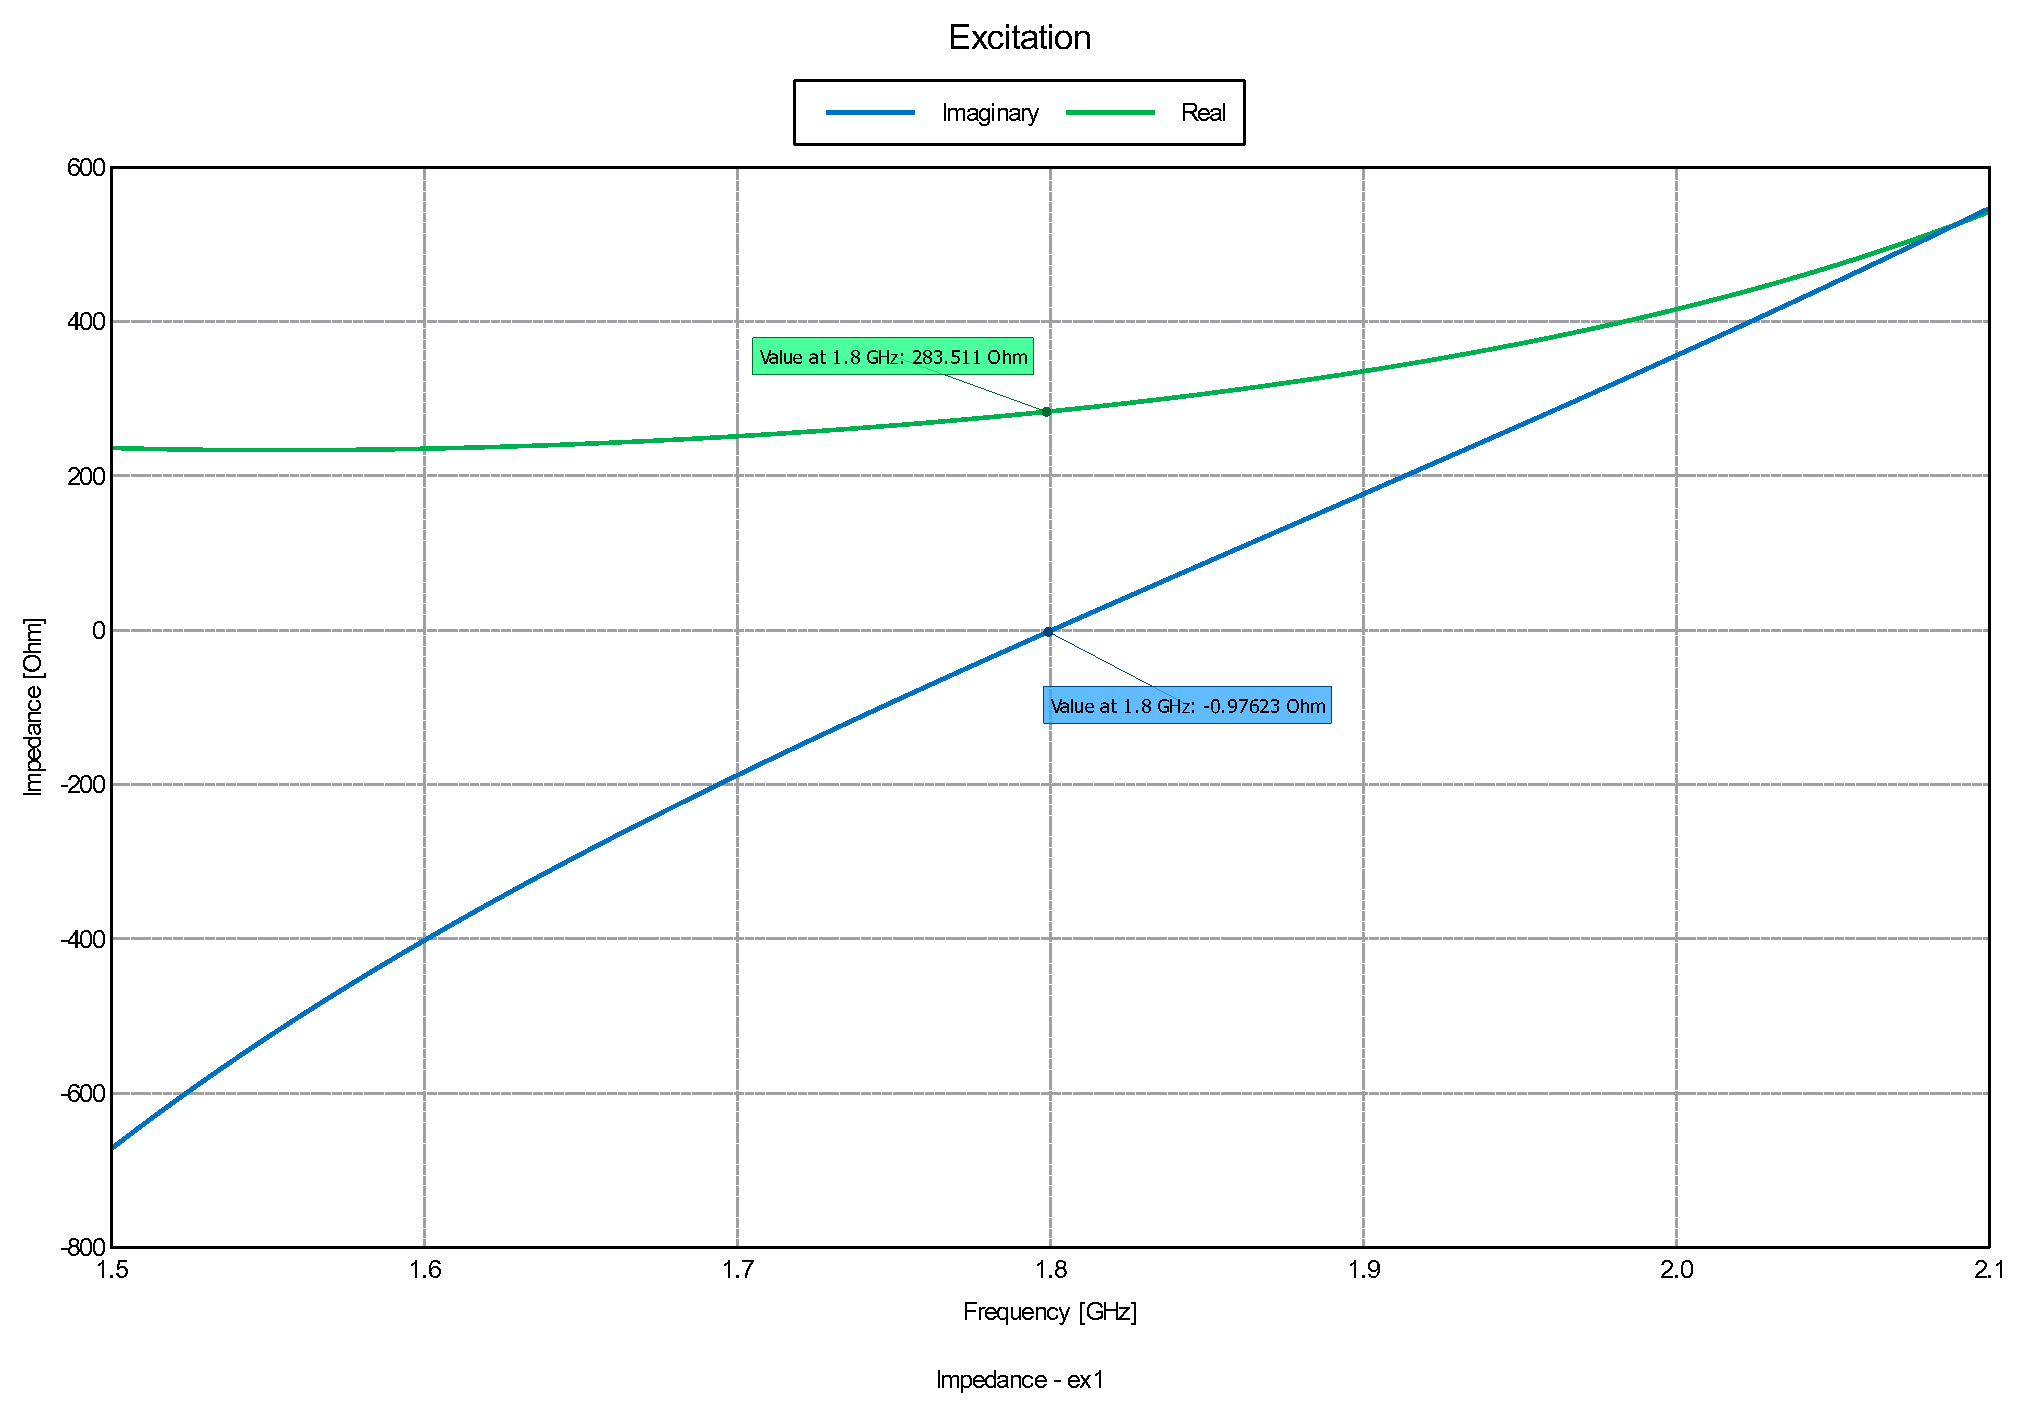
\includegraphics[width = \textwidth]{Z232.pdf}
  \caption{$\Im(Z_L)$ en fonction du dipôle replié adapté pour \SI{1.8}{\giga\hertz}.\label{fig:Z232}}
\end{figure}
Sur la figure \ref{fig:Z232}, on constate aussi que la partie réelle de l'impédance du dipôle replié est près de 4 fois supérieure à la partie réelle de l'impédance du dipôle demi-onde.

Le coefficient de réflexion de ce dipôle replié est représenté en fonction de la fréquence à la figure \ref{fig:gamma23},
\begin{figure}[htbp]
  \centering
  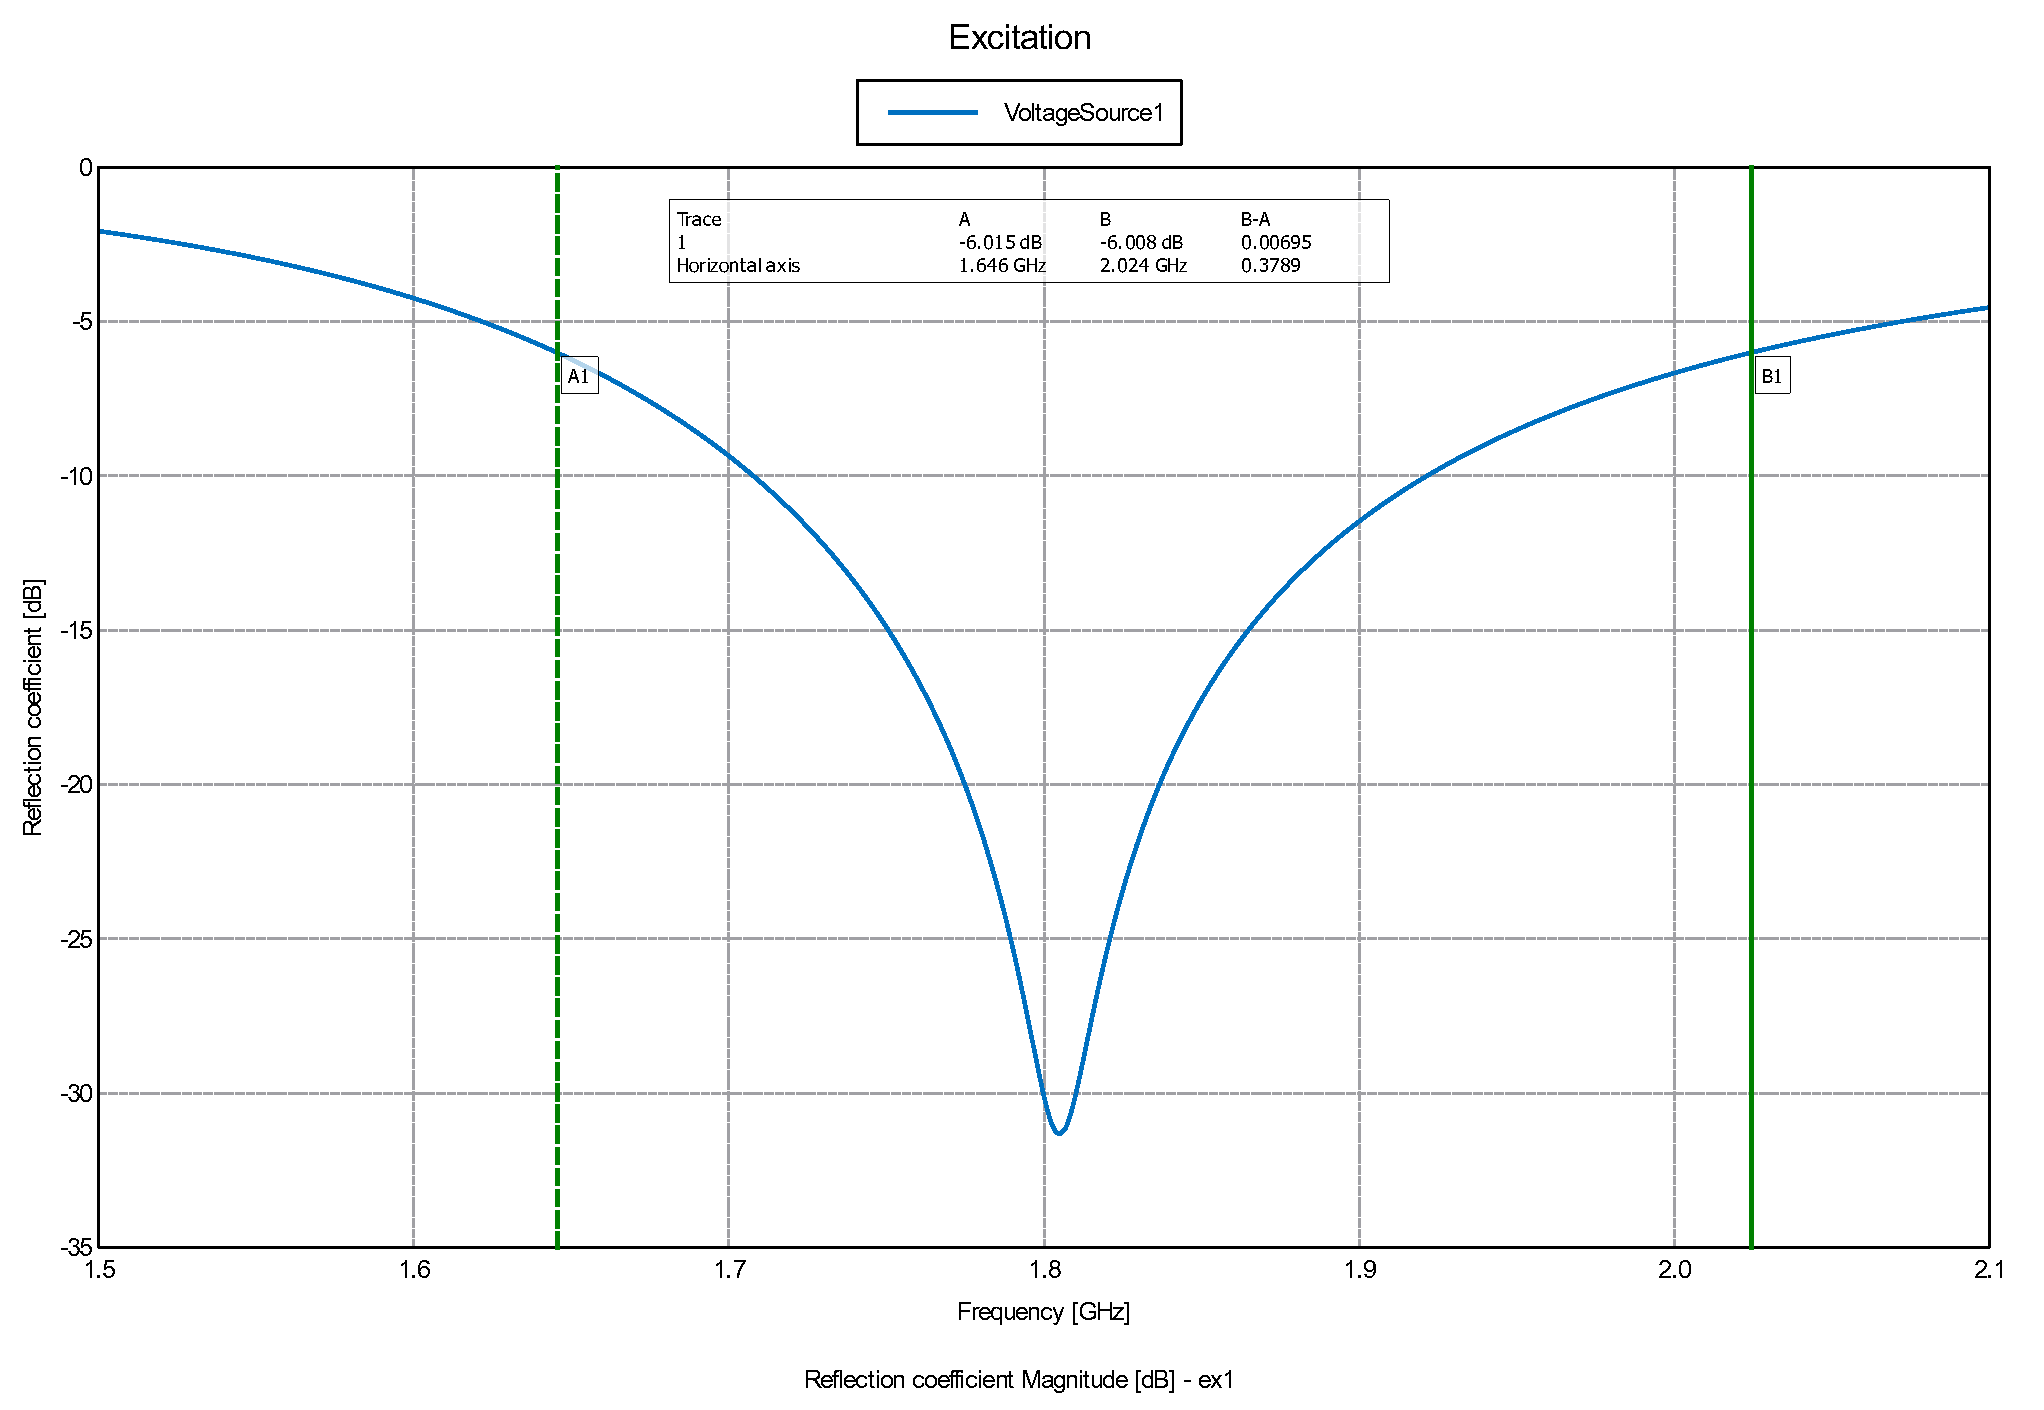
\includegraphics[width = \textwidth]{gamma23.pdf}
  \caption{$\Gamma_L$ du dipôle replié en fonction de la fréquence}
\end{figure}
pour une source d'impédance \SI{300}{\ohm}. Sur cette figure, on lit $\Gamma_L \simeq \SI{-30}{\deci\bel}$ à \SI{1.8}{\giga\hertz} et une largeur de bande de \SI{379}{\mega\hertz}. La largeur de bande à donc augmenté de plus de \SI{50}{\percent} par rapport à celle du dipôle demi-onde de même diamètre ($0.00001\lambda$).

Le gain est représenté dans un diagramme polaire à la figure \ref{fig:gain234}.
\begin{figure}[htbp]
  \centering
  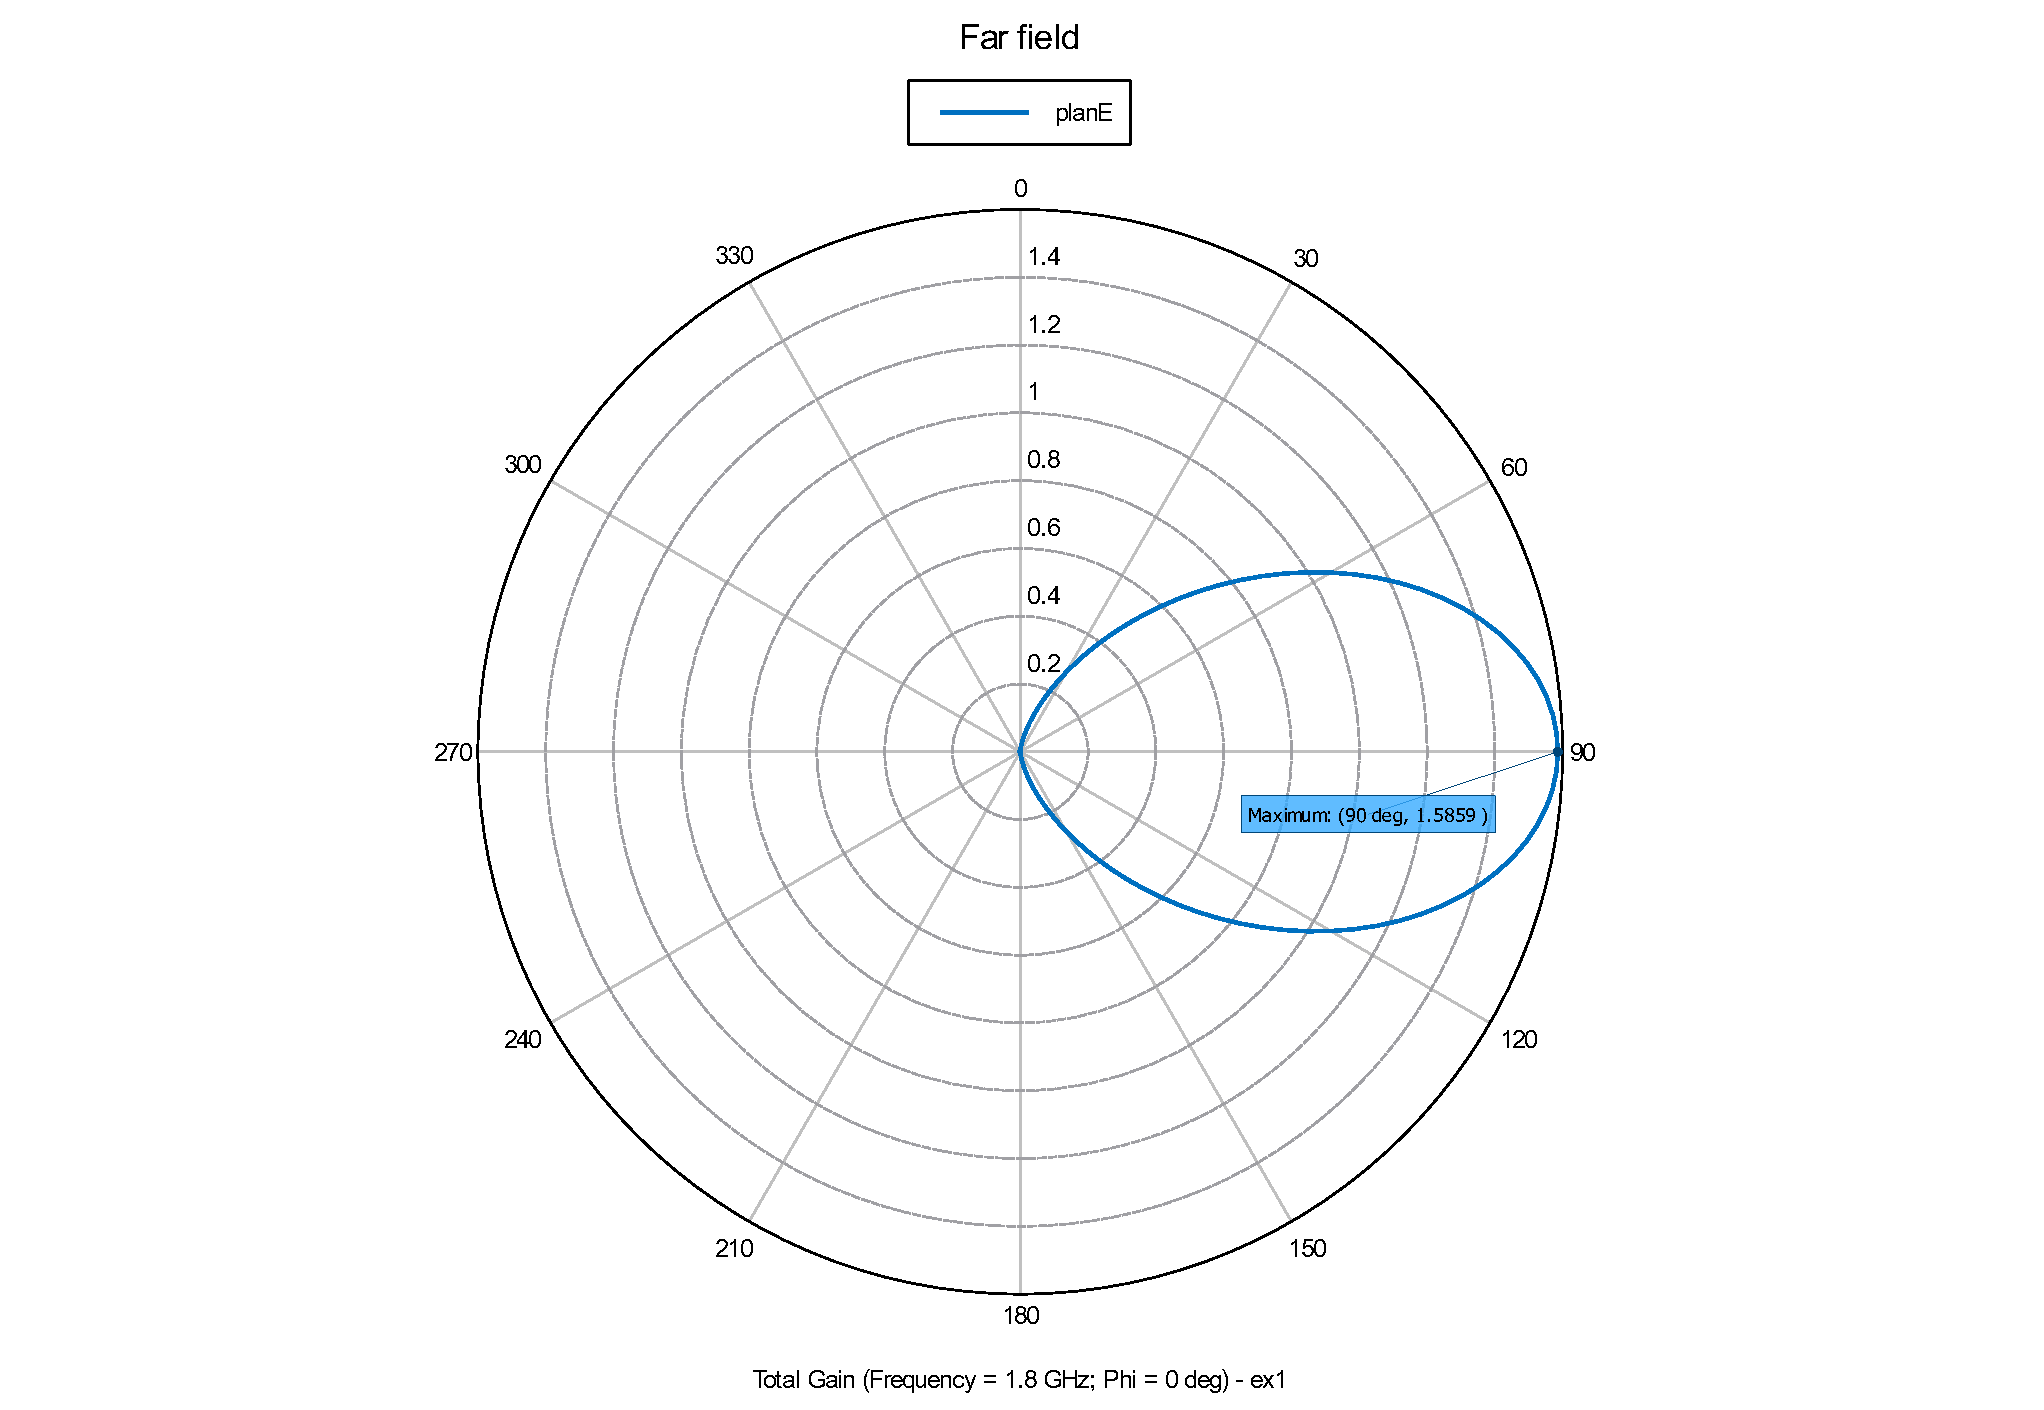
\includegraphics[width = \textwidth]{gain234.pdf}
  \caption{Diagramme polaire du gain du dipôle replié dans le plan E.\label{fig:gain234}}
\end{figure}
Le gain maximal est toujours bien évidemment dans le plan $\theta = 0$ et vaut \num{1.56}, ce qui est légèrement inférieur au gain maximal du dipôle demi-onde.

\subsection{Réseau de dipôles}
Nous étudions ici la mise en série de 4 dipôles demi-onde dont la longueur est telle que $\Im(Z_L)=0$ (voir section \ref{subsec:demionde}). Pour avoir une direction maximale de rayonnement en $\theta=\frac{2\pi}{3}$, on peut évaluer le déphasage nécessaire entre chaque source par la relation \ref{eqn:dephasage}
\begin{equation}\label{eqn:dephasage}
\delta = \beta d \cos(\theta)
\end{equation}
Où $\beta = \frac{2\pi f}{c} = $ est le nombre d'onde et $d$, la distance entre deux sources.

Suite à cela, nous avons simulé le système : on peut constater sur la figure \ref{fig:rayonnement4} que le gain maximum est de $\num{4.24} = \SI{6.27}{\deci\bel}$.

\begin{figure}[htbp]
  \centering
  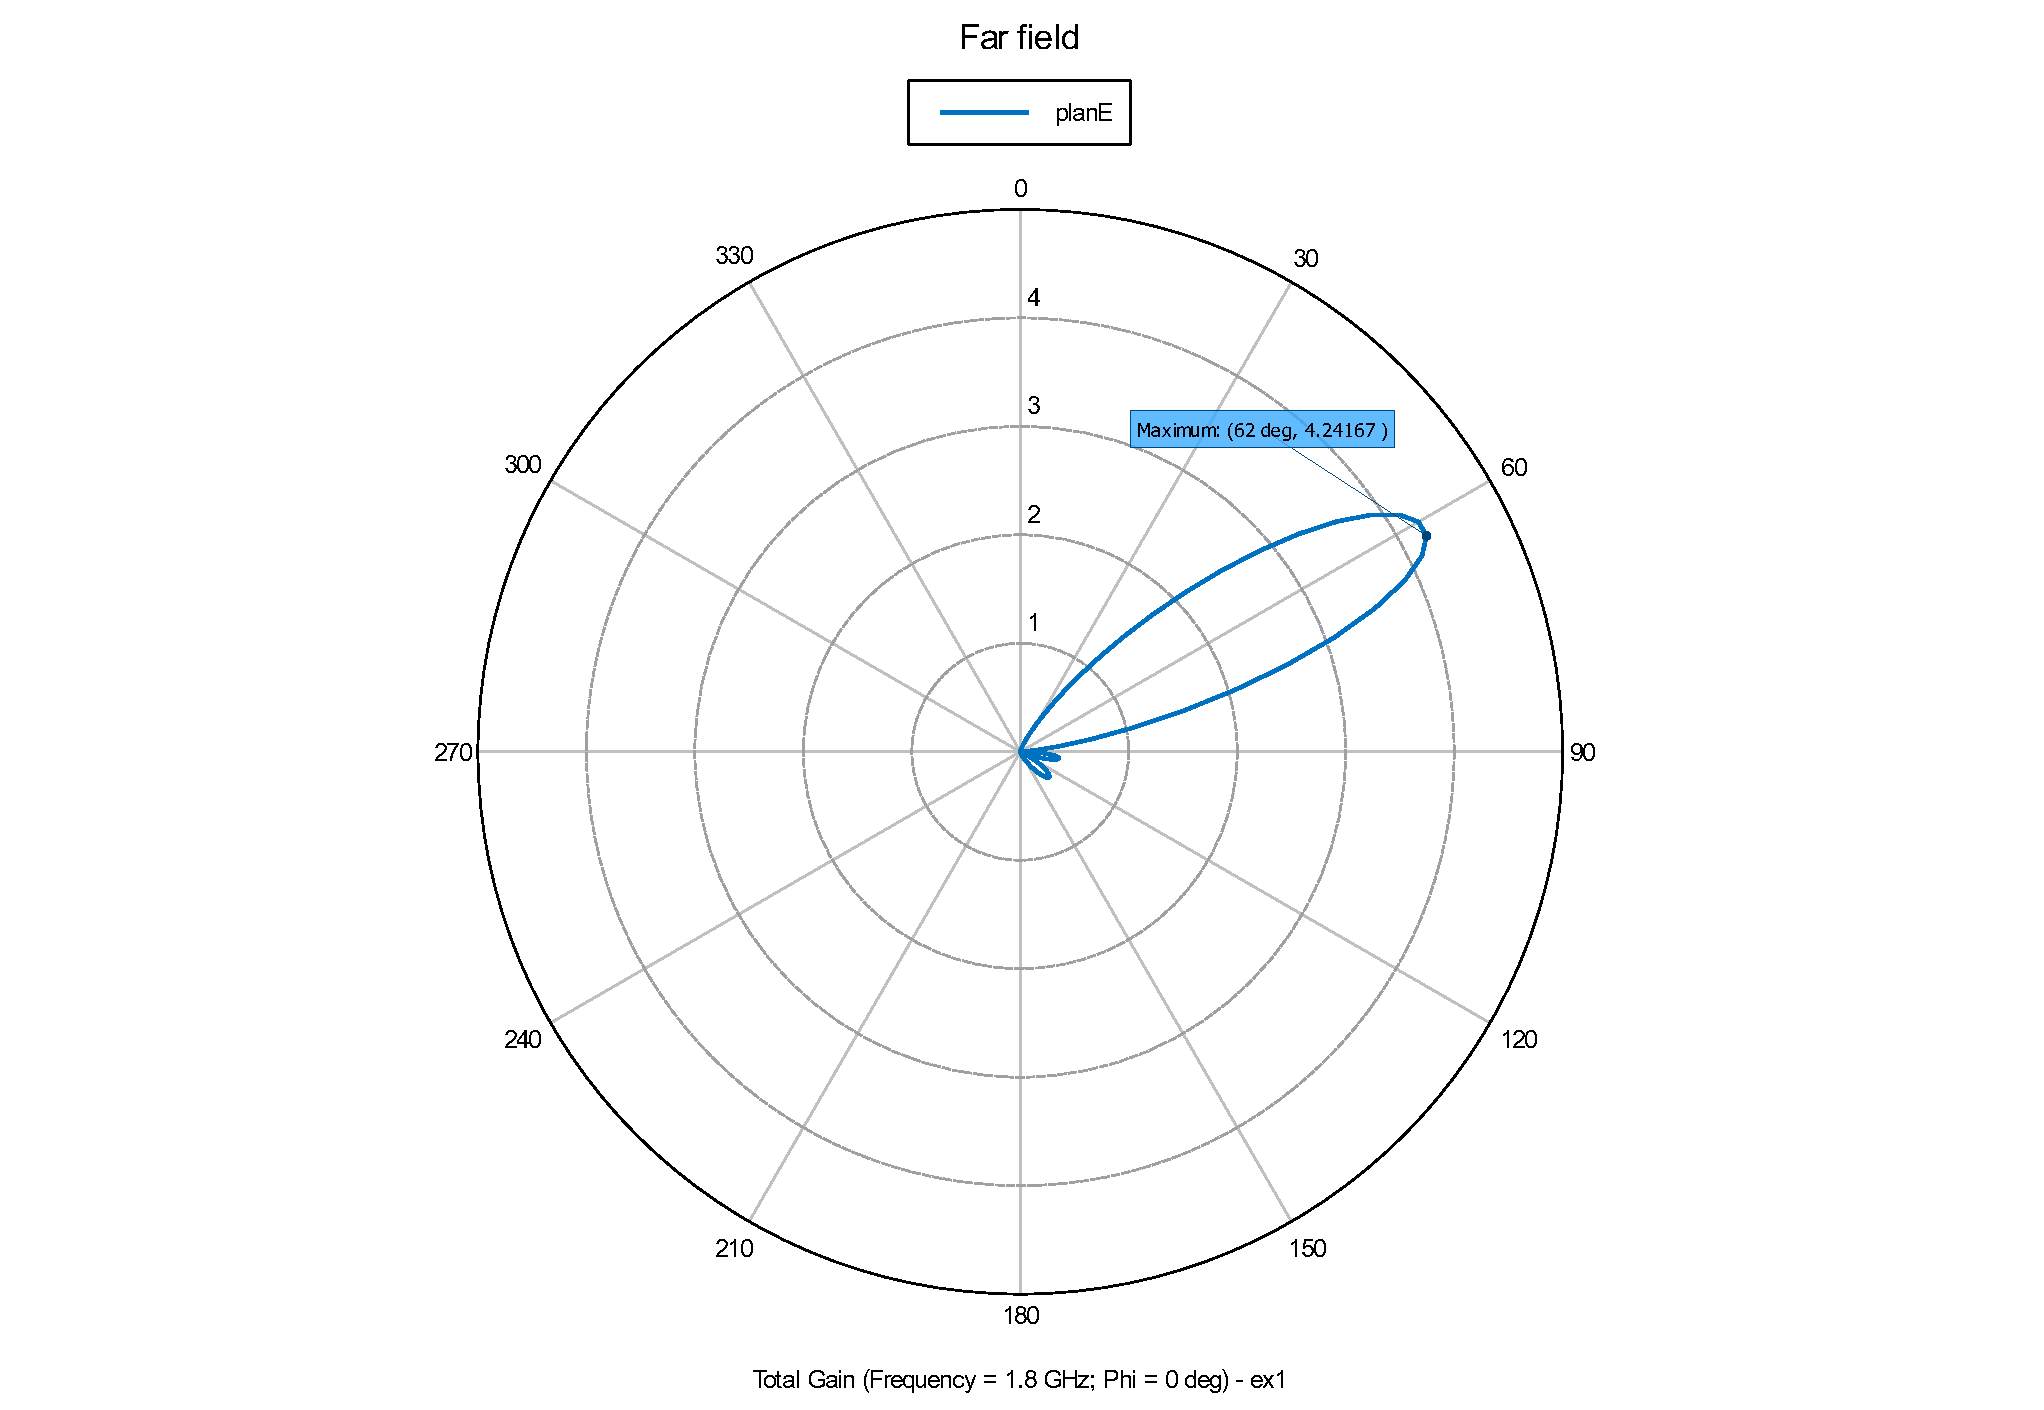
\includegraphics[width = \textwidth]{rayonnement24.pdf}
  \caption{Diagramme de rayonnement du réseau de dipôles demi-onde dans le plan E\label{fig:rayonnement4}}
\end{figure}

Nous avons ensuite rajouté au système un plan conducteur parfait de dimension $3\lambda \times \lambda$ parallèle à l'axe des dipôles et à une distance $\frac{\lambda}{4}$ de ceux-ci. Après une seconde simulation, on peut constater un gain de $\num{14} = \SI{11.46}{\deci\bel}$ sur la figure \ref{fig:rayonnement4reflecteur}, ce qui est nettement mieux que sans le plan réflecteur. Ceci s'explique par le fait que le réseau ne rayonne plus en direction du plan et, par conséquent, rayonne plus fortement dans les autres directions.

\begin{figure}[htbp]
  \centering
  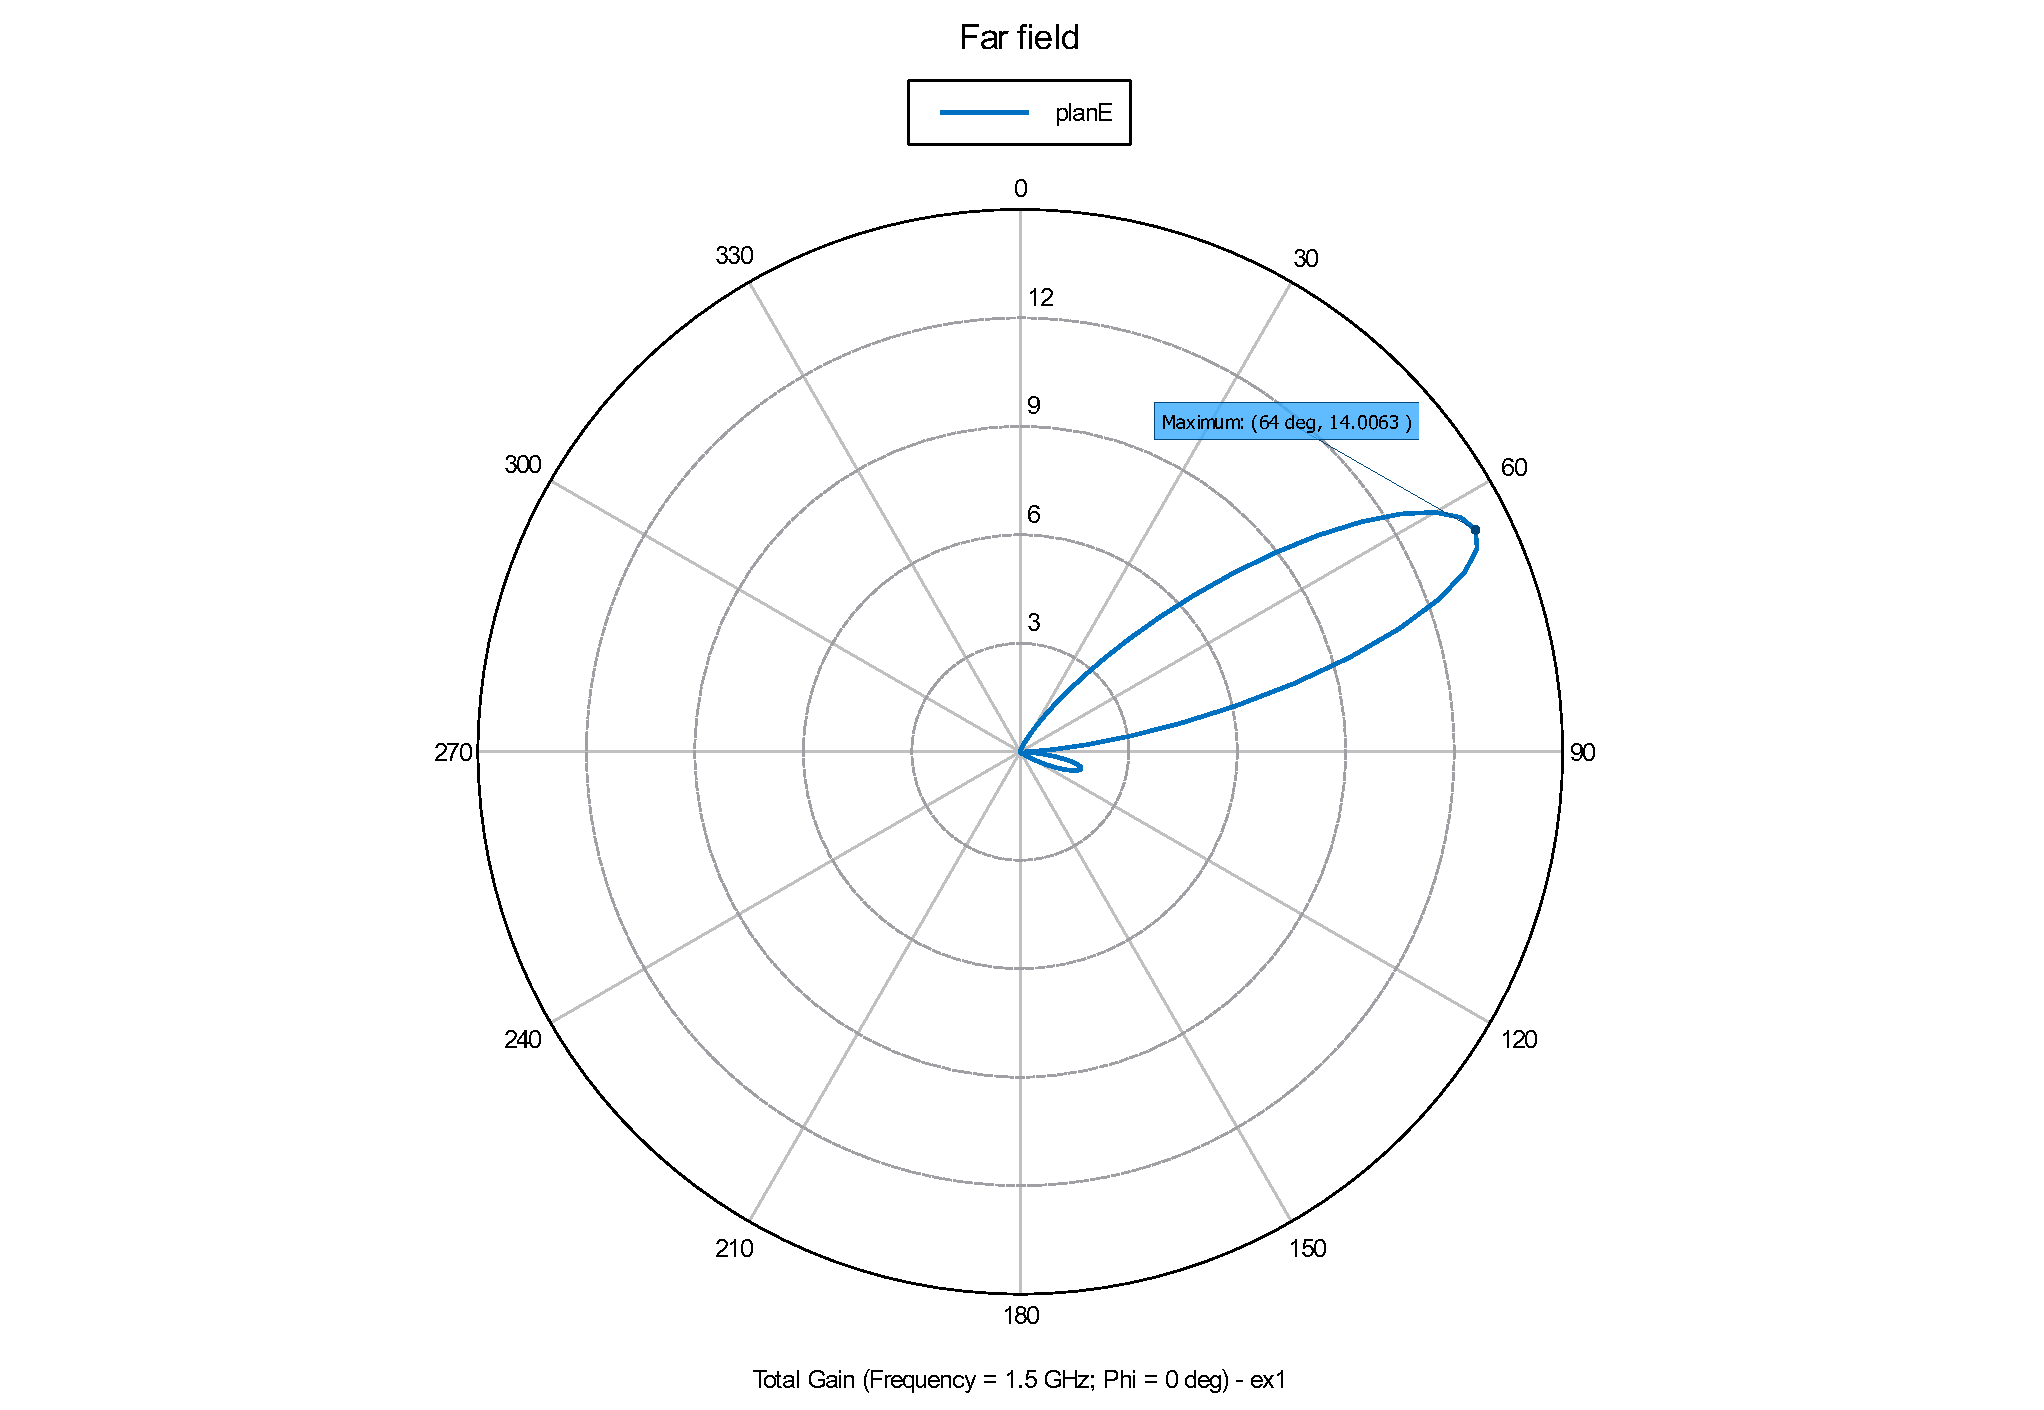
\includegraphics[width = \textwidth]{rayonnement24b.pdf}
  \caption{Diagramme de rayonnement du réseau de dipôles demi-onde avec un plan réflecteur dans le plan E\label{fig:rayonnement4reflecteur}}
\end{figure}

Nous pouvons comparer les trois configurations étudiées du dipôle demi-onde : le dipôle seul,le réseau sans réflecteur et avec réflecteur :

\begin{tabular}{|l|c|r|}
  \hline
       dipôle demi-onde & Réseau sans réflecteur & réseau avec réflecteur \\
  \hline
  $\SI{1.79}{\deci\bel}$ & $\SI{6.27}{\deci\bel}$ & $\SI{11.46}{\deci\bel}$ \\
  \hline
\end{tabular}

%Coucou jason! Attention qu'une ligne vide = 1 nouveau paragraphe=> une idée séparée. Si tu veux absolument mettre des lignes vides autour de figures dans le code, mets les en commentaire.



%Représentation de 2 en float 64bits. Maintenant je peux noter mes labos de 4.9406564584124654 × 10^−324 à 1.7976931348623157 × 10^308.
%QUESTCE QUE TU VA FAIIIIIIIIIIIIIIIIIIIIIIIIIIRE?

%bite

%roi du game

%jt bz


\end{document}